%\documentclass[class=article,crop=false, multi=true]{standalone}
%% **************************************************************************************************************
\RequirePackage{fix-cm} % fix some latex issues see: http://texdoc.net/texmf-dist/doc/latex/base/fixltx2e.pdf
\documentclass[ twoside,openright,titlepage,numbers=noenddot,headinclude,%1headlines,% letterpaper a4paper
                footinclude=true,cleardoublepage=empty,abstractoff, % <--- obsolete, remove (todo)
                BCOR=5mm,paper=a4,fontsize=11pt,%11pt,a4paper,%
                ngerman,american,%
                ]{scrreprt}


%********************************************************************
% Note: Make all your adjustments in here
%*******************************************************
% ****************************************************************************************************
% classicthesis-config.tex 
% formerly known as loadpackages.sty, classicthesis-ldpkg.sty, and classicthesis-preamble.sty 
% Use it at the beginning of your ClassicThesis.tex, or as a LaTeX Preamble 
% in your ClassicThesis.{tex,lyx} with % ****************************************************************************************************
% classicthesis-config.tex 
% formerly known as loadpackages.sty, classicthesis-ldpkg.sty, and classicthesis-preamble.sty 
% Use it at the beginning of your ClassicThesis.tex, or as a LaTeX Preamble 
% in your ClassicThesis.{tex,lyx} with \input{classicthesis-config}
% ****************************************************************************************************  
% If you like the classicthesis, then I would appreciate a postcard. 
% My address can be found in the file ClassicThesis.pdf. A collection 
% of the postcards I received so far is available online at 
% http://postcards.miede.de
% ****************************************************************************************************


% ****************************************************************************************************
% 0. Set the encoding of your files. UTF-8 is the only sensible encoding nowadays. If you can't read
% äöüßáéçèê∂åëæƒÏ€ then change the encoding setting in your editor, not the line below. If your editor
% does not support utf8 use another editor!
% ****************************************************************************************************
\PassOptionsToPackage{utf8}{inputenc}
	\usepackage{inputenc}

% ****************************************************************************************************
% 1. Configure classicthesis for your needs here, e.g., remove "drafting" below 
% in order to deactivate the time-stamp on the pages
% ****************************************************************************************************
\PassOptionsToPackage{eulerchapternumbers,listings,drafting,%
					 pdfspacing,%floatperchapter,%linedheaders,%
					 subfig,beramono,eulermath,parts,dottedtoc}{classicthesis}                                        
% ********************************************************************
% Available options for classicthesis.sty 
% (see ClassicThesis.pdf for more information):
% drafting
% parts nochapters linedheaders
% eulerchapternumbers beramono eulermath pdfspacing minionprospacing
% tocaligned dottedtoc manychapters
% listings floatperchapter subfig
% ********************************************************************


% ****************************************************************************************************
% 2. Personal data and user ad-hoc commands
% ****************************************************************************************************
\newcommand{\myTitle}{Internal Variability of carbon sink in Southern Ocean\xspace}
\newcommand{\myName}{Aaron Spring\xspace}
\newcommand{\myProf}{Prof. Dr. Norbert Frank\xspace}
\newcommand{\mySecondProf}{Prof. Dr. Johanna Baehr\xspace}
\newcommand{\mySecondProfInstitution}{University of Hamburg, Department of Oceanography\xspace}
\newcommand{\mySupervisor}{Dr. Tatiana Ilyina\xspace}
\newcommand{\myFaculty}{Faculty of Physics and Astronomy\xspace}
\newcommand{\myFacultyGerman}{Fakultät für Physik und Astronomie\xspace}
\newcommand{\myDepartment}{Environmental Physics\xspace}
\newcommand{\myDepartmentGerman}{Umweltphysik\xspace}
\newcommand{\myUni}{Ruprecht-Karls-University Heidelberg\xspace}
\newcommand{\myUniGerman}{Ruprecht-Karls-Universität Heidelberg\xspace}
\newcommand{\myLocation}{Heidelberg\xspace}
\newcommand{\myTime}{June 2017\xspace}
\newcommand{\myThesisYear}{2017}
\newcommand{\myBirthday}{14 February 1990\xspace}
\newcommand{\myBirthdayGerman}{14. Februar 1990\xspace}
\newcommand{\myBirthplace}{Frankfurt\xspace}

\newcommand{\myVersion}{version 0.1\xspace}

% ********************************************************************
% Setup, finetuning, and useful commands
% ********************************************************************
\newcounter{dummy} % necessary for correct hyperlinks (to index, bib, etc.)
\newlength{\abcd} % for ab..z string length calculation
\providecommand{\mLyX}{L\kern-.1667em\lower.25em\hbox{Y}\kern-.125emX\@}
\newcommand{\ie}{i.\,e.}
\newcommand{\Ie}{I.\,e.}
\newcommand{\eg}{e.\,g.}
\newcommand{\Eg}{E.\,g.} 
% ****************************************************************************************************


% ****************************************************************************************************
% 3. Loading some handy packages
% ****************************************************************************************************
% ******************************************************************** 
% Packages with options that might require adjustments
% ******************************************************************** 
%\PassOptionsToPackage{ngerman,american}{babel}   % change this to your language(s)
% Spanish languages need extra options in order to work with this template
%\PassOptionsToPackage{spanish,es-lcroman}{babel}
	\usepackage{babel}                  

%\usepackage[square]{natbib}
\usepackage{csquotes}
\PassOptionsToPackage{%
    %backend=biber, %instead of bibtex
	backend=bibtex8,bibencoding=ascii,%
	language=auto,%
	%style=numeric-comp,%
    style=authoryear-comp, % Author 1999, 2010
    %bibstyle=authoryear, %dashed=false, % dashed: substitute rep. author with ---
	%citestyle=authoryear-comp,    
    sorting=nyt, % name, year, title
    maxbibnames=10, % default: 3, et al.
    %backref=true,%
    natbib=true % natbib compatibility mode (\citep and \citet still work)
}{biblatex}
    \usepackage{biblatex}


\PassOptionsToPackage{fleqn}{amsmath}       % math environments and more by the AMS 
    \usepackage{amsmath}

% ******************************************************************** 
% General useful packages
% ******************************************************************** 
\PassOptionsToPackage{T1}{fontenc} % T2A for cyrillics
    \usepackage{fontenc}     
\usepackage{textcomp} % fix warning with missing font shapes
\usepackage{scrhack} % fix warnings when using KOMA with listings package          
\usepackage{xspace} % to get the spacing after macros right  
\usepackage{mparhack} % get marginpar right
\usepackage{fixltx2e} % fixes some LaTeX stuff --> since 2015 in the LaTeX kernel (see below)
%\usepackage[latest]{latexrelease} % will be used once available in more distributions (ISSUE #107)
\PassOptionsToPackage{printonlyused,smaller}{acronym} 
    \usepackage{acronym} % nice macros for handling all acronyms in the thesis
    %\renewcommand{\bflabel}[1]{{#1}\hfill} % fix the list of acronyms --> no longer working
    %\renewcommand*{\acsfont}[1]{\textsc{#1}} 
    \renewcommand*{\aclabelfont}[1]{\acsfont{#1}}
% ****************************************************************************************************


% ****************************************************************************************************
% 4. Setup floats: tables, (sub)figures, and captions
% ****************************************************************************************************
\usepackage{tabularx} % better tables
    \setlength{\extrarowheight}{3pt} % increase table row height
\newcommand{\tableheadline}[1]{\multicolumn{1}{c}{\spacedlowsmallcaps{#1}}}
\newcommand{\myfloatalign}{\centering} % to be used with each float for alignment
\usepackage{caption}
% Thanks to cgnieder and Claus Lahiri
% http://tex.stackexchange.com/questions/69349/spacedlowsmallcaps-in-caption-label
% [REMOVED DUE TO OTHER PROBLEMS, SEE ISSUE #82]    
%\DeclareCaptionLabelFormat{smallcaps}{\bothIfFirst{#1}{~}\MakeTextLowercase{\textsc{#2}}}
%\captionsetup{font=small,labelformat=smallcaps} % format=hang,
\captionsetup{font=small} % format=hang,
\usepackage{subfig}  
% ****************************************************************************************************


% ****************************************************************************************************
% 5. Setup code listings
% ****************************************************************************************************
\usepackage{listings} 
%\lstset{emph={trueIndex,root},emphstyle=\color{BlueViolet}}%\underbar} % for special keywords
\lstset{language=[LaTeX]Tex,%C++,
    morekeywords={PassOptionsToPackage,selectlanguage},
    keywordstyle=\color{RoyalBlue},%\bfseries,
    basicstyle=\small\ttfamily,
    %identifierstyle=\color{NavyBlue},
    commentstyle=\color{Green}\ttfamily,
    stringstyle=\rmfamily,
    numbers=none,%left,%
    numberstyle=\scriptsize,%\tiny
    stepnumber=5,
    numbersep=8pt,
    showstringspaces=false,
    breaklines=true,
    %frameround=ftff,
    %frame=single,
    belowcaptionskip=.75\baselineskip
    %frame=L
} 
% ****************************************************************************************************             


% ****************************************************************************************************
% 6. PDFLaTeX, hyperreferences and citation backreferences
% ****************************************************************************************************
% ********************************************************************
% Using PDFLaTeX
% ********************************************************************
\PassOptionsToPackage{pdftex,hyperfootnotes=false,pdfpagelabels}{hyperref}
    \usepackage{hyperref}  % backref linktocpage pagebackref
\pdfcompresslevel=9
\pdfadjustspacing=1 
\PassOptionsToPackage{pdftex}{graphicx}
    \usepackage{graphicx} 
 

% ********************************************************************
% Hyperreferences
% ********************************************************************
\hypersetup{%
    %draft, % = no hyperlinking at all (useful in b/w printouts)
    colorlinks=true, linktocpage=true, pdfstartpage=1, pdfstartview=FitV,%
    % uncomment the following line if you want to have black links (e.g., for printing)
    %colorlinks=false, linktocpage=false, pdfstartpage=3, pdfstartview=FitV, pdfborder={0 0 0},%
    breaklinks=true, pdfpagemode=UseNone, pageanchor=true, pdfpagemode=UseOutlines,%
    plainpages=false, bookmarksnumbered, bookmarksopen=true, bookmarksopenlevel=1,%
    hypertexnames=true, pdfhighlight=/O,%nesting=true,%frenchlinks,%
    urlcolor=webblack, linkcolor=RoyalBlue, citecolor=webgreen, %pagecolor=RoyalBlue,%
    %urlcolor=Black, linkcolor=Black, citecolor=Black, %pagecolor=Black,%
    pdftitle={\myTitle},%
    pdfauthor={\textcopyright\ \myName, \myUni, \myFaculty},%
    pdfsubject={},%
    pdfkeywords={},%
    pdfcreator={pdfLaTeX},%
    pdfproducer={LaTeX with hyperref and classicthesis}%
}   

% ********************************************************************
% Setup autoreferences
% ********************************************************************
% There are some issues regarding autorefnames
% http://www.ureader.de/msg/136221647.aspx
% http://www.tex.ac.uk/cgi-bin/texfaq2html?label=latexwords
% you have to redefine the makros for the 
% language you use, e.g., american, ngerman
% (as chosen when loading babel/AtBeginDocument)
% ********************************************************************
\makeatletter
\@ifpackageloaded{babel}%
    {%
       \addto\extrasamerican{%
			\renewcommand*{\figureautorefname}{Figure}%
			\renewcommand*{\tableautorefname}{Table}%
			\renewcommand*{\partautorefname}{Part}%
			\renewcommand*{\chapterautorefname}{Chapter}%
			\renewcommand*{\sectionautorefname}{Section}%
			\renewcommand*{\subsectionautorefname}{Section}%
			\renewcommand*{\subsubsectionautorefname}{Section}%     
                }%
       \addto\extrasngerman{% 
			\renewcommand*{\paragraphautorefname}{Absatz}%
			\renewcommand*{\subparagraphautorefname}{Unterabsatz}%
			\renewcommand*{\footnoteautorefname}{Fu\"snote}%
			\renewcommand*{\FancyVerbLineautorefname}{Zeile}%
			\renewcommand*{\theoremautorefname}{Theorem}%
			\renewcommand*{\appendixautorefname}{Anhang}%
			\renewcommand*{\equationautorefname}{Gleichung}%        
			\renewcommand*{\itemautorefname}{Punkt}%
                }%  
            % Fix to getting autorefs for subfigures right (thanks to Belinda Vogt for changing the definition)
            \providecommand{\subfigureautorefname}{\figureautorefname}%             
    }{\relax}
\makeatother


% ****************************************************************************************************
% 7. Last calls before the bar closes
% ****************************************************************************************************
% ********************************************************************
% Development Stuff
% ********************************************************************
\listfiles
%\PassOptionsToPackage{l2tabu,orthodox,abort}{nag}
%   \usepackage{nag}
%\PassOptionsToPackage{warning, all}{onlyamsmath}
%   \usepackage{onlyamsmath}

% ********************************************************************
% Last, but not least...
% ********************************************************************
\usepackage{classicthesis} 
% ****************************************************************************************************


% ****************************************************************************************************
% 8. Further adjustments (experimental)
% ****************************************************************************************************
% ********************************************************************
% Changing the text area
% ********************************************************************
%\linespread{1.05} % a bit more for Palatino
%\areaset[current]{312pt}{761pt} % 686 (factor 2.2) + 33 head + 42 head \the\footskip
%\setlength{\marginparwidth}{7em}%
%\setlength{\marginparsep}{2em}%

% ********************************************************************
% Using different fonts
% ********************************************************************
%\usepackage[oldstylenums]{kpfonts} % oldstyle notextcomp
%\usepackage[osf]{libertine}
%\usepackage[light,condensed,math]{iwona}
%\renewcommand{\sfdefault}{iwona}
%\usepackage{lmodern} % <-- no osf support :-(
%\usepackage{cfr-lm} % 
%\usepackage[urw-garamond]{mathdesign} <-- no osf support :-(
%\usepackage[default,osfigures]{opensans} % scale=0.95 
%\usepackage[sfdefault]{FiraSans}
% ****************************************************************************************************

% ****************************************************************************************************  
% If you like the classicthesis, then I would appreciate a postcard. 
% My address can be found in the file ClassicThesis.pdf. A collection 
% of the postcards I received so far is available online at 
% http://postcards.miede.de
% ****************************************************************************************************


% ****************************************************************************************************
% 0. Set the encoding of your files. UTF-8 is the only sensible encoding nowadays. If you can't read
% äöüßáéçèê∂åëæƒÏ€ then change the encoding setting in your editor, not the line below. If your editor
% does not support utf8 use another editor!
% ****************************************************************************************************
\PassOptionsToPackage{utf8}{inputenc}
	\usepackage{inputenc}

% ****************************************************************************************************
% 1. Configure classicthesis for your needs here, e.g., remove "drafting" below 
% in order to deactivate the time-stamp on the pages
% ****************************************************************************************************
\PassOptionsToPackage{eulerchapternumbers,listings,drafting,%
					 pdfspacing,%floatperchapter,%linedheaders,%
					 subfig,beramono,eulermath,parts,dottedtoc}{classicthesis}                                        
% ********************************************************************
% Available options for classicthesis.sty 
% (see ClassicThesis.pdf for more information):
% drafting
% parts nochapters linedheaders
% eulerchapternumbers beramono eulermath pdfspacing minionprospacing
% tocaligned dottedtoc manychapters
% listings floatperchapter subfig
% ********************************************************************


% ****************************************************************************************************
% 2. Personal data and user ad-hoc commands
% ****************************************************************************************************
\newcommand{\myTitle}{Internal Variability of carbon sink in Southern Ocean\xspace}
\newcommand{\myName}{Aaron Spring\xspace}
\newcommand{\myProf}{Prof. Dr. Norbert Frank\xspace}
\newcommand{\mySecondProf}{Prof. Dr. Johanna Baehr\xspace}
\newcommand{\mySecondProfInstitution}{University of Hamburg, Department of Oceanography\xspace}
\newcommand{\mySupervisor}{Dr. Tatiana Ilyina\xspace}
\newcommand{\myFaculty}{Faculty of Physics and Astronomy\xspace}
\newcommand{\myFacultyGerman}{Fakultät für Physik und Astronomie\xspace}
\newcommand{\myDepartment}{Environmental Physics\xspace}
\newcommand{\myDepartmentGerman}{Umweltphysik\xspace}
\newcommand{\myUni}{Ruprecht-Karls-University Heidelberg\xspace}
\newcommand{\myUniGerman}{Ruprecht-Karls-Universität Heidelberg\xspace}
\newcommand{\myLocation}{Heidelberg\xspace}
\newcommand{\myTime}{June 2017\xspace}
\newcommand{\myThesisYear}{2017}
\newcommand{\myBirthday}{14 February 1990\xspace}
\newcommand{\myBirthdayGerman}{14. Februar 1990\xspace}
\newcommand{\myBirthplace}{Frankfurt\xspace}

\newcommand{\myVersion}{version 0.1\xspace}

% ********************************************************************
% Setup, finetuning, and useful commands
% ********************************************************************
\newcounter{dummy} % necessary for correct hyperlinks (to index, bib, etc.)
\newlength{\abcd} % for ab..z string length calculation
\providecommand{\mLyX}{L\kern-.1667em\lower.25em\hbox{Y}\kern-.125emX\@}
\newcommand{\ie}{i.\,e.}
\newcommand{\Ie}{I.\,e.}
\newcommand{\eg}{e.\,g.}
\newcommand{\Eg}{E.\,g.} 
% ****************************************************************************************************


% ****************************************************************************************************
% 3. Loading some handy packages
% ****************************************************************************************************
% ******************************************************************** 
% Packages with options that might require adjustments
% ******************************************************************** 
%\PassOptionsToPackage{ngerman,american}{babel}   % change this to your language(s)
% Spanish languages need extra options in order to work with this template
%\PassOptionsToPackage{spanish,es-lcroman}{babel}
	\usepackage{babel}                  

%\usepackage[square]{natbib}
\usepackage{csquotes}
\PassOptionsToPackage{%
    %backend=biber, %instead of bibtex
	backend=bibtex8,bibencoding=ascii,%
	language=auto,%
	%style=numeric-comp,%
    style=authoryear-comp, % Author 1999, 2010
    %bibstyle=authoryear, %dashed=false, % dashed: substitute rep. author with ---
	%citestyle=authoryear-comp,    
    sorting=nyt, % name, year, title
    maxbibnames=10, % default: 3, et al.
    %backref=true,%
    natbib=true % natbib compatibility mode (\citep and \citet still work)
}{biblatex}
    \usepackage{biblatex}


\PassOptionsToPackage{fleqn}{amsmath}       % math environments and more by the AMS 
    \usepackage{amsmath}

% ******************************************************************** 
% General useful packages
% ******************************************************************** 
\PassOptionsToPackage{T1}{fontenc} % T2A for cyrillics
    \usepackage{fontenc}     
\usepackage{textcomp} % fix warning with missing font shapes
\usepackage{scrhack} % fix warnings when using KOMA with listings package          
\usepackage{xspace} % to get the spacing after macros right  
\usepackage{mparhack} % get marginpar right
\usepackage{fixltx2e} % fixes some LaTeX stuff --> since 2015 in the LaTeX kernel (see below)
%\usepackage[latest]{latexrelease} % will be used once available in more distributions (ISSUE #107)
\PassOptionsToPackage{printonlyused,smaller}{acronym} 
    \usepackage{acronym} % nice macros for handling all acronyms in the thesis
    %\renewcommand{\bflabel}[1]{{#1}\hfill} % fix the list of acronyms --> no longer working
    %\renewcommand*{\acsfont}[1]{\textsc{#1}} 
    \renewcommand*{\aclabelfont}[1]{\acsfont{#1}}
% ****************************************************************************************************


% ****************************************************************************************************
% 4. Setup floats: tables, (sub)figures, and captions
% ****************************************************************************************************
\usepackage{tabularx} % better tables
    \setlength{\extrarowheight}{3pt} % increase table row height
\newcommand{\tableheadline}[1]{\multicolumn{1}{c}{\spacedlowsmallcaps{#1}}}
\newcommand{\myfloatalign}{\centering} % to be used with each float for alignment
\usepackage{caption}
% Thanks to cgnieder and Claus Lahiri
% http://tex.stackexchange.com/questions/69349/spacedlowsmallcaps-in-caption-label
% [REMOVED DUE TO OTHER PROBLEMS, SEE ISSUE #82]    
%\DeclareCaptionLabelFormat{smallcaps}{\bothIfFirst{#1}{~}\MakeTextLowercase{\textsc{#2}}}
%\captionsetup{font=small,labelformat=smallcaps} % format=hang,
\captionsetup{font=small} % format=hang,
\usepackage{subfig}  
% ****************************************************************************************************


% ****************************************************************************************************
% 5. Setup code listings
% ****************************************************************************************************
\usepackage{listings} 
%\lstset{emph={trueIndex,root},emphstyle=\color{BlueViolet}}%\underbar} % for special keywords
\lstset{language=[LaTeX]Tex,%C++,
    morekeywords={PassOptionsToPackage,selectlanguage},
    keywordstyle=\color{RoyalBlue},%\bfseries,
    basicstyle=\small\ttfamily,
    %identifierstyle=\color{NavyBlue},
    commentstyle=\color{Green}\ttfamily,
    stringstyle=\rmfamily,
    numbers=none,%left,%
    numberstyle=\scriptsize,%\tiny
    stepnumber=5,
    numbersep=8pt,
    showstringspaces=false,
    breaklines=true,
    %frameround=ftff,
    %frame=single,
    belowcaptionskip=.75\baselineskip
    %frame=L
} 
% ****************************************************************************************************             


% ****************************************************************************************************
% 6. PDFLaTeX, hyperreferences and citation backreferences
% ****************************************************************************************************
% ********************************************************************
% Using PDFLaTeX
% ********************************************************************
\PassOptionsToPackage{pdftex,hyperfootnotes=false,pdfpagelabels}{hyperref}
    \usepackage{hyperref}  % backref linktocpage pagebackref
\pdfcompresslevel=9
\pdfadjustspacing=1 
\PassOptionsToPackage{pdftex}{graphicx}
    \usepackage{graphicx} 
 

% ********************************************************************
% Hyperreferences
% ********************************************************************
\hypersetup{%
    %draft, % = no hyperlinking at all (useful in b/w printouts)
    colorlinks=true, linktocpage=true, pdfstartpage=1, pdfstartview=FitV,%
    % uncomment the following line if you want to have black links (e.g., for printing)
    %colorlinks=false, linktocpage=false, pdfstartpage=3, pdfstartview=FitV, pdfborder={0 0 0},%
    breaklinks=true, pdfpagemode=UseNone, pageanchor=true, pdfpagemode=UseOutlines,%
    plainpages=false, bookmarksnumbered, bookmarksopen=true, bookmarksopenlevel=1,%
    hypertexnames=true, pdfhighlight=/O,%nesting=true,%frenchlinks,%
    urlcolor=webblack, linkcolor=RoyalBlue, citecolor=webgreen, %pagecolor=RoyalBlue,%
    %urlcolor=Black, linkcolor=Black, citecolor=Black, %pagecolor=Black,%
    pdftitle={\myTitle},%
    pdfauthor={\textcopyright\ \myName, \myUni, \myFaculty},%
    pdfsubject={},%
    pdfkeywords={},%
    pdfcreator={pdfLaTeX},%
    pdfproducer={LaTeX with hyperref and classicthesis}%
}   

% ********************************************************************
% Setup autoreferences
% ********************************************************************
% There are some issues regarding autorefnames
% http://www.ureader.de/msg/136221647.aspx
% http://www.tex.ac.uk/cgi-bin/texfaq2html?label=latexwords
% you have to redefine the makros for the 
% language you use, e.g., american, ngerman
% (as chosen when loading babel/AtBeginDocument)
% ********************************************************************
\makeatletter
\@ifpackageloaded{babel}%
    {%
       \addto\extrasamerican{%
			\renewcommand*{\figureautorefname}{Figure}%
			\renewcommand*{\tableautorefname}{Table}%
			\renewcommand*{\partautorefname}{Part}%
			\renewcommand*{\chapterautorefname}{Chapter}%
			\renewcommand*{\sectionautorefname}{Section}%
			\renewcommand*{\subsectionautorefname}{Section}%
			\renewcommand*{\subsubsectionautorefname}{Section}%     
                }%
       \addto\extrasngerman{% 
			\renewcommand*{\paragraphautorefname}{Absatz}%
			\renewcommand*{\subparagraphautorefname}{Unterabsatz}%
			\renewcommand*{\footnoteautorefname}{Fu\"snote}%
			\renewcommand*{\FancyVerbLineautorefname}{Zeile}%
			\renewcommand*{\theoremautorefname}{Theorem}%
			\renewcommand*{\appendixautorefname}{Anhang}%
			\renewcommand*{\equationautorefname}{Gleichung}%        
			\renewcommand*{\itemautorefname}{Punkt}%
                }%  
            % Fix to getting autorefs for subfigures right (thanks to Belinda Vogt for changing the definition)
            \providecommand{\subfigureautorefname}{\figureautorefname}%             
    }{\relax}
\makeatother


% ****************************************************************************************************
% 7. Last calls before the bar closes
% ****************************************************************************************************
% ********************************************************************
% Development Stuff
% ********************************************************************
\listfiles
%\PassOptionsToPackage{l2tabu,orthodox,abort}{nag}
%   \usepackage{nag}
%\PassOptionsToPackage{warning, all}{onlyamsmath}
%   \usepackage{onlyamsmath}

% ********************************************************************
% Last, but not least...
% ********************************************************************
\usepackage{classicthesis} 
% ****************************************************************************************************


% ****************************************************************************************************
% 8. Further adjustments (experimental)
% ****************************************************************************************************
% ********************************************************************
% Changing the text area
% ********************************************************************
%\linespread{1.05} % a bit more for Palatino
%\areaset[current]{312pt}{761pt} % 686 (factor 2.2) + 33 head + 42 head \the\footskip
%\setlength{\marginparwidth}{7em}%
%\setlength{\marginparsep}{2em}%

% ********************************************************************
% Using different fonts
% ********************************************************************
%\usepackage[oldstylenums]{kpfonts} % oldstyle notextcomp
%\usepackage[osf]{libertine}
%\usepackage[light,condensed,math]{iwona}
%\renewcommand{\sfdefault}{iwona}
%\usepackage{lmodern} % <-- no osf support :-(
%\usepackage{cfr-lm} % 
%\usepackage[urw-garamond]{mathdesign} <-- no osf support :-(
%\usepackage[default,osfigures]{opensans} % scale=0.95 
%\usepackage[sfdefault]{FiraSans}
% ****************************************************************************************************


\usepackage{graphicx}
\usepackage{indentfirst}
\graphicspath{{/home/mpim/m300524/MSc_Thesis/gfx/}}

\newrobustcmd*{\parentexttrack}[1]{%
  \begingroup
  \blx@blxinit
  \blx@setsfcodes
  \blx@bibopenparen#1\blx@bibcloseparen
  \endgroup}

\AtEveryCite{%
  \let\parentext=\parentexttrack%
  \let\bibopenparen=\bibopenbracket%
  \let\bibcloseparen=\bibclosebracket}

%********************************************************************
% Bibliographies
%*******************************************************
%\addbibresource{Bibliography.bib}
%\addbibresource{AMiede_Publications.bib}
%\bibliographystyle{apalike}
%\addbibresource{SouthernOceanCarbonSink.bib}
\bibliography{Paper/SouthernOceanCarbonSink_new.bib}
%\bibliographystyle{abbrvnat}
%********************************************************************
% Hyphenation
%*******************************************************
%\hyphenation{put special hyphenation here}

% ********************************************************************
% GO!GO!GO! MOVE IT!
%*******************************************************
\begin{document}
\frenchspacing
\raggedbottom
\selectlanguage{american} % american ngerman
%\renewcommand*{\bibname}{new name}
%\setbibpreamble{}
\pagenumbering{roman}
\pagestyle{plain}
%********************************************************************
% Frontmatter
%*******************************************************
%\includegraphics[scale=1,page=2]{coffee.pdf}
%*******************************************************
% Titlepage
%*******************************************************
\begin{titlepage}
    % if you want the titlepage to be centered, uncomment and fine-tune the line below (KOMA classes environment)
    \begin{addmargin}[-1cm]{-3cm}
    \renewcommand{\baselinestretch}{2.00}
    \begin{center}
        \Large  

		\myFaculty \\
		\smallskip
		
		\large
		\myUni

        \hfill

        \vfill

    	\medskip
		
        \vfill
		Master thesis \\ 
		in Physics \\ 
		submitted by \\ 
		\myName \\ 
		born in \myBirthplace  \\
		\myThesisYear 
        
%        \vfill                      

    \end{center}  
  \end{addmargin}    

  
\cleardoublepage  
\begin{center}
  \renewcommand{\baselinestretch}{2.00}
  \Large \bfseries%\sffamily
    \myTitle 
    
  \par
  \vfill
  \large\normalfont
  This Master thesis has been carried out by \myName \\
  at the institute of \myDepartment \\
  under the supervision of \\
  \myProf \\%(Frau/Herrn Prof./Priv.-Doz. Name Surname)
  %% additionally insert second supervisor here if carrying out an
  %% external diploma thesis. Reduce vspace in L. 44 accordingly.
  and \\ 
  \mySecondProf  \\ from \\ \mySecondProfInstitution 
\end{center}\par
\vspace{5\baselineskip}

% reset baselinestretch
\renewcommand{\baselinestretch}{1.00}\normalsize  
  
  
  
     
\end{titlepage}   
\cleardoublepage
%*******************************************************
% Abstract
%*******************************************************
%\renewcommand{\abstractname}{Abstract}
\pdfbookmark[1]{Abstract}{Abstract}
%\begingroup
%\let\clearpage\relax
%\let\cleardoublepage\relax
%\let\cleardoublepage\relax

\chapter*{Abstract}
%The Southern Ocean is a major sink for anthropogenic CO$_2$ emissions and hence it plays an essential role in modulating global carbon cycle and climate change. Previous studies based on observations show pronounced decadal variations of carbon uptake in the Southern Ocean in recent decades and this variability is largely driven by internal climate variability. However, due to limited ensemble size of simulations, the variability of this important ocean sink is still poorly assessed by the state-of-the-art earth system models (ESMs). To assess the internal variability of carbon sink in the Southern Ocean, we use a large ensemble of 100 member simulations based on the Max Planck Institute-ESM (MPI-ESM). Here we use model simulations from 1980-2015 to compare with available observation-based dataset. We found several ensemble members showing decadal trends in the carbon sink, which are similar to the trends shown in observations. This result suggests that MPI-ESM large ensemble simulations are able to reproduce decadal variation of carbon sink in the Southern Ocean. Moreover, the trends of Southern Ocean carbon sink in MPI-ESM are mainly contributed by region between 50-60$^\circ$S. %To understand the internal variability of the sea-air carbon fluxes in the Southern Ocean, we further investigate the variability of underlying processes, such as physical climate variability and ocean biological processes. 
%Our results focus on the impact of biology on decadal trends of carbon sink. Primary production in area from 50-60$^\circ$S is very sensible to euphotic water column stability. Changes in the physical state of the water column influence biological drawdown of ocean surface pCO$_2$ and hence the Southern Ocean carbon sink.
Recent observations suggest pronounced decadal variations in the Southern Ocean carbon sink. However, due to the sparse spatial and temporal coverage of observations, it is challenging to discern the dynamics of internally varying processes. Earth system models (ESMs), while being a useful tool to analyze processes that contribute to variability, rarely capture this variability in a small ensemble size. I assess modeled decadal internal variability by analyzing a large ensemble of 100 historical simulations based on Max Planck Institute's ESM (MPI-ESM) starting from different initial conditions but using identical forcing.

The modeled decadal internal variability of the Southern Ocean carbon sink south of 35$^\circ$S is quantified to be $\sim\pm0.19$ PgC/yr/decade in the historical period. This amounts to $\sim12\%$ of the mean state of carbon sink at $\sim1.15$ PgC/yr and dominates over the forced signal of $\sim-0.14$ PgC/yr/decade. MPI-ESM Large Ensemble captures decadal variations of similar magnitude as suggested by observations. The largest variability is found at 50-60$^\circ$S, where CO$_2$ flux follows two wind-driven regimes: stronger winds enhance the upper-ocean overturning circulation and the corresponding upwelling of deep waters weakens the carbon sink. For weakening winds, the upper-ocean circulation slows down and hence strengthens the carbon sink.



%\vfill
\clearpage

\begin{otherlanguage}{ngerman}
\pdfbookmark[1]{Zusammenfassung}{Zusammenfassung}
\chapter*{Zusammenfassung}
%Neue Beobachtungsdaten zeigen dekadische Schwankungen in der Kohlenstoffsenke im Südlichen Ozean auf. Die spärliche räumliche und temporäre Beobachtungsdatendichte macht das Unterscheiden der Dynamik der variablen Prozesse herausfordernd. Erdsystemmodelle, die ein nützliches Hilfsmittel zum Analysieren von variablen Prozessen sind, erfassen selten diese internen Schwankungen. Durch das Analysieren eines Ensembles mit 100 historischen Simulationen basierend auf dem Max-Planck-Institut ESM (MPI-ESM) mit leicht veränderten Anfangsbedingungen untersuche ich modellierte interne Variabilität. 

%Die modellierte dekadische interne Variabilität der Kohlenstoffsenke im Südlichen Ozean südlich von 35$^\circ$S beträgt $\sim\pm0.19$ PgC/Jahr/Dekade. Dies macht $\sim12\%$ der durchschnittlichen Kohlenstoffaufnahme von $\sim-1.15$ PgC/Jahr aus und dominiert über das erzwungene Klimawandelsignal von $\sim-0.14$ PgC/Jahr/Dekade. Die 100 MPI-ESM Simulationen erfassen dekadische Trends von ähnlicher Stärke im Vergleich mit Beobachtungsdaten. In der Region mit der höchsten Variabilität bei 50-60$^\circ$S ergeben sich zwei wind-getriebene Regime: Stärkere Winde stimulieren die obere Umwelzzirkulation, was das Aufsteigen von Tiefenwasser verstärkt. Das darauf folgene Ausgasen reduziert die Kohlenstoffsenke. Schwächere Wind reduzieren die Umwelzzirkulation und stärken somit die Kohlenstoffsenke.
%// sollte kuerzer als 200 Worte sein

In kürzlich veröffentlichen Beobachtungsdaten lassen sich dekadische Schwankungen in der Kohlenstoffsenke im Südlichen Ozean erkennen. Dabei stellt es sich aufgrund der geringen räumlichen und temporären Beobachtungsdatendichte als schwierig dar, die Dynamik der variablen Prozesse zu unterscheiden. Erdsystemmodelle, die ein nützliches Hilfsmittel zur Analyse von variablen Prozessen sind, erfassen diese internen Schwankungen nur selten. In der vorliegenden Masterarbeit untersuche ich modellierte interne Variabilität mittels Analyse eines Ensembles von 100 historischen Simulationen,
basierend auf dem Max-Planck-Institut ESM (MPI-ESM) mit leicht
veränderten Anfangsbedingungen.

Die modellierte dekadische interne Variabilität der Kohlenstoffsenke im Südlichen Ozean südlich von 35$^\circ$S beträgt $\sim\pm0.19$ PgC/Jahr/ Dekade. Dies macht $\sim12$\% der durchschnittlichen Kohlenstoffaufnahme von $\sim1.15$ PgC/Jahr aus und dominiert über das erzwungene Klimawandelsignal von $\sim -0.14$ PgC/Jahr/Dekade. Die 100 MPI-ESM Simulationen erfassen dekadische Trends von ähnlicher Stärke vergleichbar mit Beobachtungsdaten. Die höchste Variabilität lässt sich in der Region 50-60$^\circ$S erkennen, wo die Kohlenstoffflüsse durch folgende zwei Windregime beeinflusst werden: herrschen stärkere Winde, stimulieren sie die obere Umwelzzirkulation, was das Aufsteigen von Tiefenwasser verstärkt und durch das darauf folgende Ausgasen die Kohlenstoffsenke reduziert; auf der anderen Seite verlangsamen schwächere Winde die Umwelzzirkulation und stärken somit die Kohlenstoffsenke.

\end{otherlanguage}

%\endgroup			

%\vfill
\pagestyle{scrheadings}
\cleardoublepage
%*******************************************************
% Table of Contents
%*******************************************************
%\phantomsection   
\refstepcounter{dummy}
\pdfbookmark[1]{\contentsname}{tableofcontents}
\setcounter{tocdepth}{2} % <-- 2 includes up to subsections in the ToC
\setcounter{secnumdepth}{3} % <-- 3 numbers up to subsubsections
\manualmark
\markboth{\spacedlowsmallcaps{\contentsname}}{\spacedlowsmallcaps{\contentsname}}
\tableofcontents 
\automark[section]{chapter}
\renewcommand{\chaptermark}[1]{\markboth{\spacedlowsmallcaps{#1}}{\spacedlowsmallcaps{#1}}}
\renewcommand{\sectionmark}[1]{\markright{\thesection\enspace\spacedlowsmallcaps{#1}}}

%here used to be list of figures and tables
%********************************************************************
% Mainmatter
%*******************************************************
\cleardoublepage
\pagenumbering{arabic}
%\setcounter{page}{90}
% use \cleardoublepage here to avoid problems with pdfbookmark
\cleardoublepage
%\part{Some Kind of Manual}
%************************************************
\chapter{Introduction}\label{ch:introduction}
%************************************************

\citep{Sabine2004} \\
\citep{landschuetzer2015}\\
\citep{LeQuere2007}\\
\citep{Sarmiento1984}\\
\citep{Lovenduski2005}\\
\citep{Lovenduski2007}\\
\citep{Lovenduski2008}\\
\citep{Hauck2013}\\
\citep{wang2012}\\
\citep{Wang2016}\\





%\cleardoublepage
%\ctparttext{You can put some informational part preamble text here.}
%\part{The Showcase}
%*****************************************
\chapter{Background}\label{ch:background}
%*****************************************
%\setcounter{figure}{10}
% \NoCaseChange{Homo Sapiens}



\section{Model description}
Previous studies assume gaussian statistics \citep{Thompson2015} \citep{Deser2012} 
The MPI-ESM version 1.1 with a low-resolution configuration (MPI-ESM-LR) is used for the large ensemble simulations \citep{Giorgetta2013}. The atmosphere component ECHAM6.3 is on a T63 grid, corresponding to 1.9$^\circ$ at the equator (better would be values of high latitudes), with 47 vertical layers up to 0.01 hPa \citep{Stevens2013}. 
Atmospheric pCO$_2$ uses prescribed and well mixed values. The carbon cycle is not coupled (so called diagnostic), so effects of changes in the terrestrial or oceanic carbon sink are not reflected in pCO$_{\text{2,atm}}$ and hence terrestrial and oceanic carbon sink can not interact.The ocean component MPI Ocean Model (MPIOM) has a horizontal resolution of 1.5$^\circ$ on average and 40 vertical levels \citep{Jungclaus2013}. The Hamburg Ocean Carbon Cycle Model (HAMOCC) \citep{Ilyina2013} represents the ocean biogeochemistry component of MPI-ESM. 

\begin{figure}[h]
	\centering 
	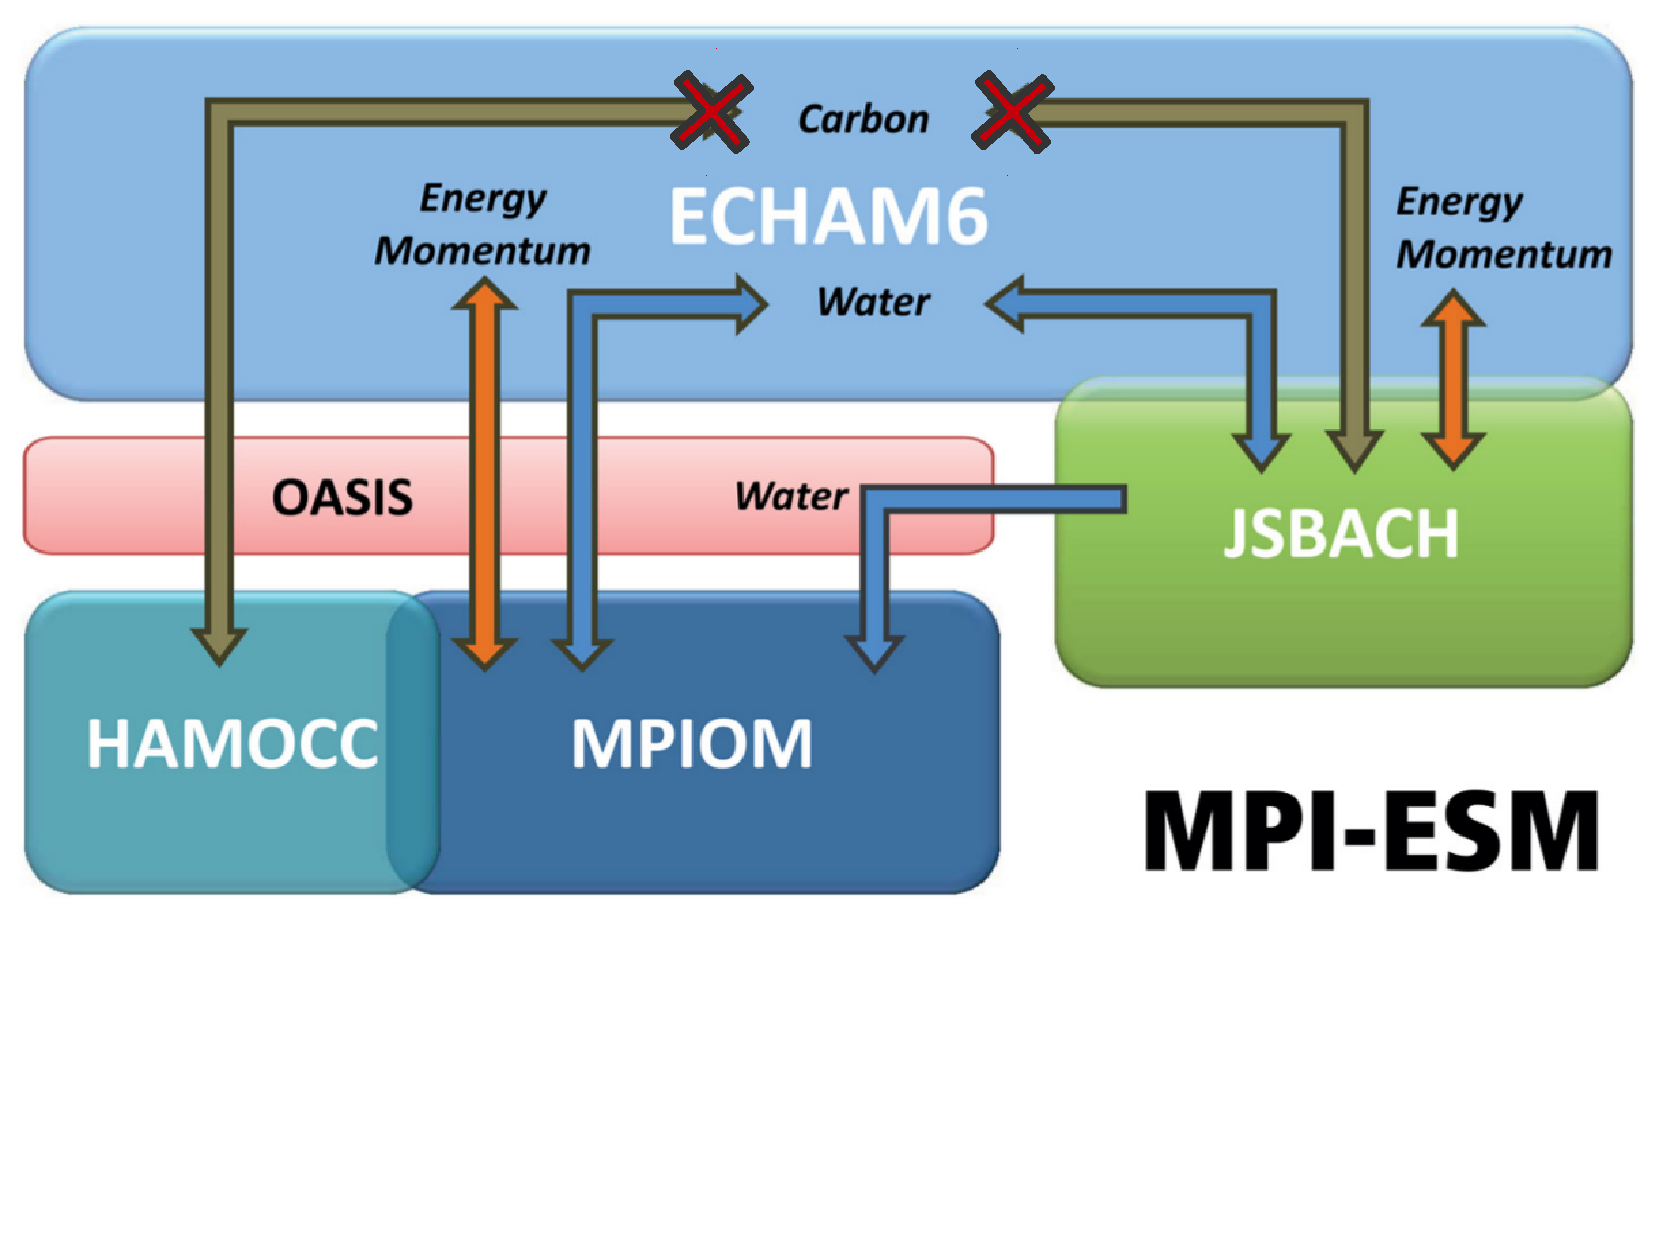
\includegraphics[scale=.42,trim=0cm 6cm 0cm 0cm,clip]{gfx/MPIESM.pdf}
	\caption{Schematic overview on the different components in MPI-Earth-System-Model}
	\label{fig:MPIESM}
\end{figure}

\subsection{HAMOCC}

\section{Large ensemble}
% about ensemble   
An ensemble of 100-member CMIP5 historical simulations and runs under  Representative Concentration Pathway (RCP) 4.5 scenario are integrated for the periods from 1850-2005, and 2006-2100, respectively. Ensemble members differ through starting from different year of the pre-industrial control simulation, so ocean and atmosphere have different initial conditions in each run.  
%ref to CESM ensemble or other ensemble studies?

\section{Fundamental processes of marine biogeochemistry}
no separation but classification, difficult to separate in nature, no single and only cause
\subsection{Physical processes}
\subsection{Biological processes}
\subsection{Chemical processes}

\section{Statistical methods}
which I used
\subsubsection*{Linear Trend}
significance via student t-test

%\subsubsection{•}

%*****************************************
%*****************************************
%*****************************************
%*****************************************
%*****************************************

%\addtocontents{toc}{\protect\clearpage} % <--- just debug stuff, ignore
%************************************************
\chapter{Math Test Chapter}\label{ch:mathtest} % $\mathbb{ZNR}$
%************************************************
Ei choro aeterno antiopam mea, labitur bonorum pri no. His no decore

\section{Some Formulas}
Due to the statistical nature of ionisation energy loss, large
lement\footnote{Examples taken from Walter Schmidt's great gallery: \\
\url{http://home.vrweb.de/~was/mathfonts.html}}.  Continuous processes
such as multiple
scattering and energy loss play a relevant role in the l
section heads. Consider the \texttt{pdfspacing} option.
\begin{equation}
\kappa =\frac{\xi}{E_{\textrm{max}}} %\mathbb{ZNR}
\end{equation}
$E_{\textrm{max}}$ is the maximum transferable energy in a single
collision with an atomic electron.
\[
E_{\textrm{max}} =\frac{2 m_{\textrm{e}} \beta^2\gamma^2 }{1 +
2\gamma m_{\textrm{e}}/m_{\textrm{x}} + \left ( m_{\textrm{e}}
/m_{\textrm{x}}\right)^2}\ ,
\]
where $\gamma = E/m_{\textrm{x}}$, $E$ is energy and
$m_{\textrm{x}}$ the mass of the incident particle,
$\beta^2 = 1 - 1/\gamma^2$ and $m_{\textrm{e}}$ is the electron mass.
$\xi$ comes from the Rutherford scattering cross section
and is defined as:
\begin{eqnarray*} \xi  = \frac{2\pi z^2 e^4 N_{\textrm{Av}} Z \rho
\delta x}{m_{\textrm{e}} \beta^2 c^2 A} =  153.4 \frac{z^2}{\beta^2}
\frac{Z}{A}
  \rho \delta x \quad\textrm{keV},
\end{eqnarray*}
where

\begin{tabular}{ll}
$z$          & charge of the incident particle \\
$N_{\textrm{Av}}$     & Avogadro's number \\
$Z$          & atomic number of the material \\
$A$          & atomic weight of the material \\
$\rho$       & density \\
$ \delta x$  & thickness of the material \\
\end{tabular}

%************************************************
%\chapter{Trends in CO$_2$ flux} % $\mathbb{ZNR}$
\chapter{Processes corresponding to multi-year trends in sea-air CO$_2$ flux}
%************************************************
\label{ch:trends}

%\section[Winds determine internal variability]{Winds determine internal variability of the Southern Ocean CO$_2$ flux}
%\section[Westerly winds and Southern Ocean CO$_2$ flux variability]{The role of westerly winds on Southern Ocean CO$_2$ flux variability}
\section{The role of westerly winds in Southern Ocean CO$_2$ flux variability}

%\paragraph{on area 50-60S as driver of Southern Ocean internal variability, correlation plots co2flux and wind trends} 
\cite{Thompson2000} and \cite{Hall2002} describe the \acf{SAM} as the most dominant mode for higher-latitude Southern Hemisphere variability. \citeauthor{Lovenduski2007} [{\color{RoyalBlue}2007}] explain the influence of the westerly winds on the Southern Ocean carbon sink. 

To further assess internal variability due to westerly winds in \acs{MPI}-\acs{ESM} this chapter discusses the effect of westerly winds on the thermal, physical and biological controls of the Southern Ocean carbon sink in \acs{HAMOCC}.\newline

I find a correlation on 8-year trends between \acs{SAM}, which describes the position and latitudinal shift of westerly winds, and the CO$_2$ flux in the area of largest decadal internal variability at 50-60$^\circ$S (\autoref{fig:scatter}). Although the CO$_2$ flux formula (\autoref{sec:HAMOCC}) also depends on the wind speed at 10m height, the driver of the changes in \autoref{fig:scatter} is not the piston velocity $k_w$, but in $\Delta \text{pCO}_2$ \citep{Lovenduski2015}. However, the magnitude of short-term variability on the timescale of days to hours depends highly on wind strength variability whereas the direction of CO$_2$ flux is independent of wind speed. This relationship reveals two distinct regimes of wind-driven CO$_2$ flux signals in this area: 

Intensified and southward-shifted winds, associated with an increasing trend in \acs{SAM}, lead to a positive CO$_2$ flux trend. This Southern Ocean carbon sink response has been suggested frequently for the observed and projected trend in \acs{SAM} \citep{LeQuere2007,Lovenduski2007,Lovenduski2008,Hauck2013,landschuetzer2015}. The related process responses corresponding to stronger winds are explained in \autoref{sec:trends_pos}.

In \acs{MPI-ESM} I also find the reverse case of weakening and northward-shifting westerly winds, associated with a negative trend in \acs{SAM}, which lead to a negative CO$_2$ flux or ocean uptake trend. The responses of processes corresponding to weaker winds are explained in \autoref{sec:trends_neg}. However, observations do not reveal a strong multi-year negative \acs{SAM} trend (\autoref{fig:evolution_SAM}). Likewise, westerly winds did not weaken but continued to increase during the negative CO$_2$ flux trend in the 2000s \citep{landschuetzer2015}. On the contrary, depending on the starting year of the trend period, the \acs{SAM} index slightly weakened in the early 2000s \citep{Marshall2003,Lovenduski2015}, and also \cite{DeVries2017} report a decline in upper-ocean overturning circulation which may be connected to strength and position of winds. \newline

The strong trends originate in strong changes of the position and strength of Southern hemisphere westerly winds and effect of those on ocean circulation. Though the parametrized eddies in \acs{MPI-ESM LE} might allow deeper mixing to sustain for multiple years and hence longer than the seasonal timescale at which the eddies would counteract those trends \citep{Thompson2011}. Only a variable definition of isopyncal thickness diffusion could parametrize the expected eddy response from high-resolution simulations \citep{Gent2011}. These enhanced eddy fluxes in a low-resolution model are discussed in \cite{Lovenduski2013}.


\begin{figure}[h!]
\centering
%		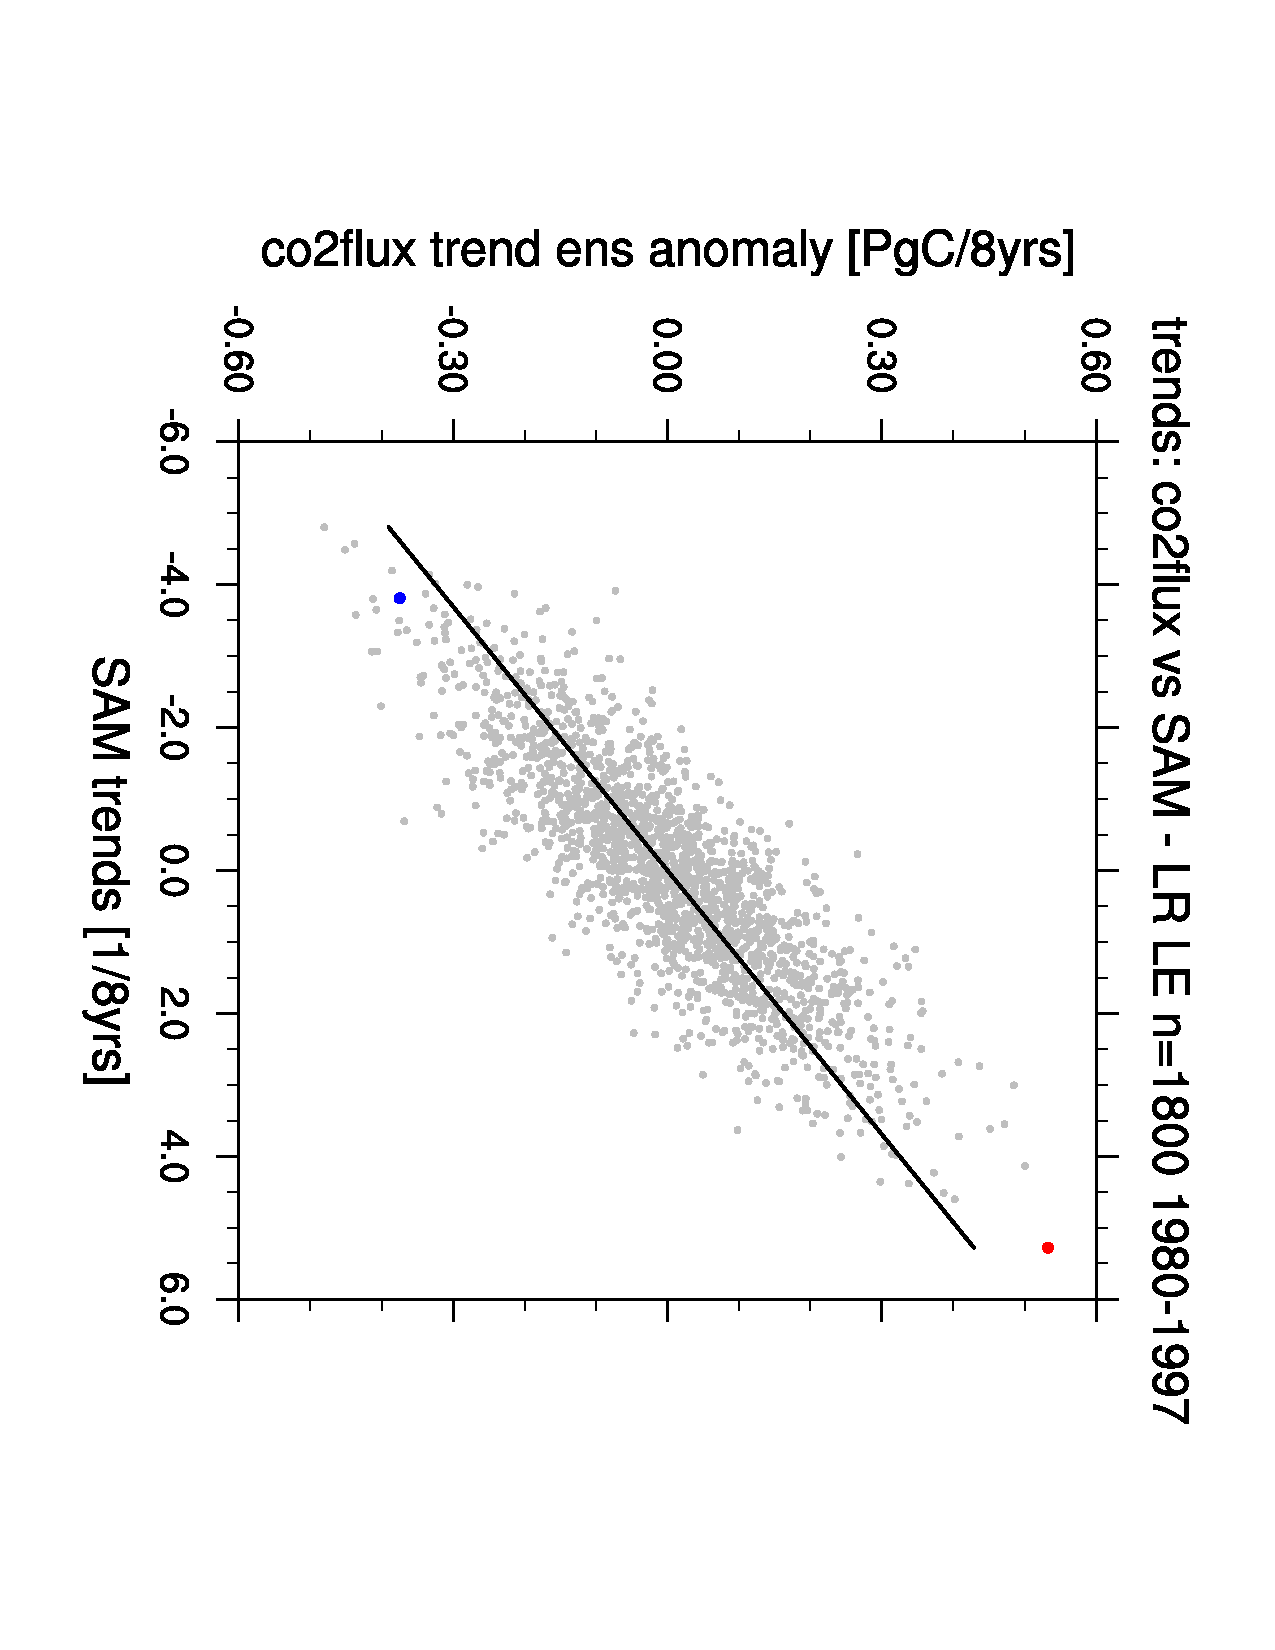
\includegraphics[scale=.5,page=1,angle=90,trim=1.3cm 2.3cm 2.3cm 3cm,clip]{Scatter_trends_bands_ensanom_co2flux_vs_SAM_n1800_1980_1997_trend8_50-59S}
		\captionsetup[subfigure]{labelformat=empty,justification=centering}
		\subfloat[Sea-air CO$_2$ vs. \acf{SAM}]{		
		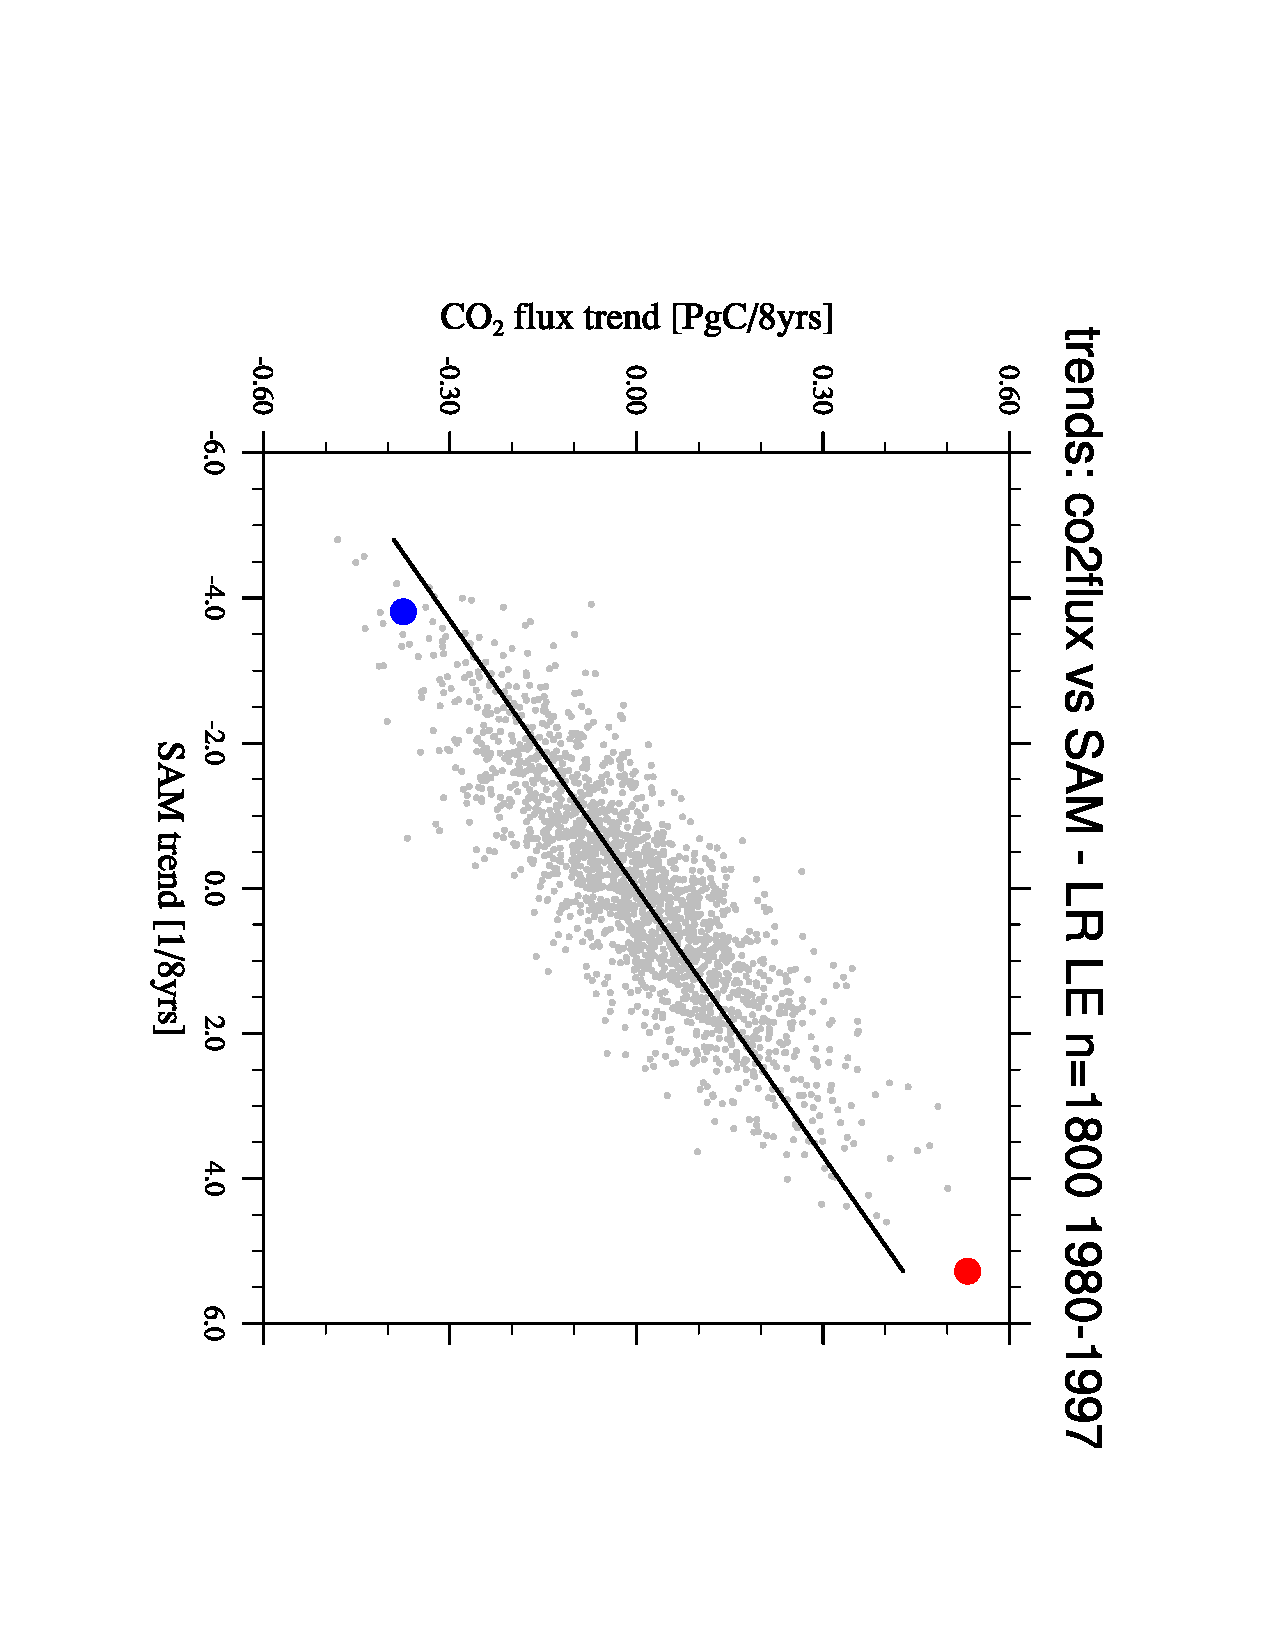
\includegraphics[scale=.6,page=1,angle=90,trim=1.3cm 2.3cm 3.8cm 4cm,clip]{EGU_new_SAM_Scatter_trends_bands_ensanom_co2flux_vs_SAM_n1800_1980_1997_trend8}}		
		%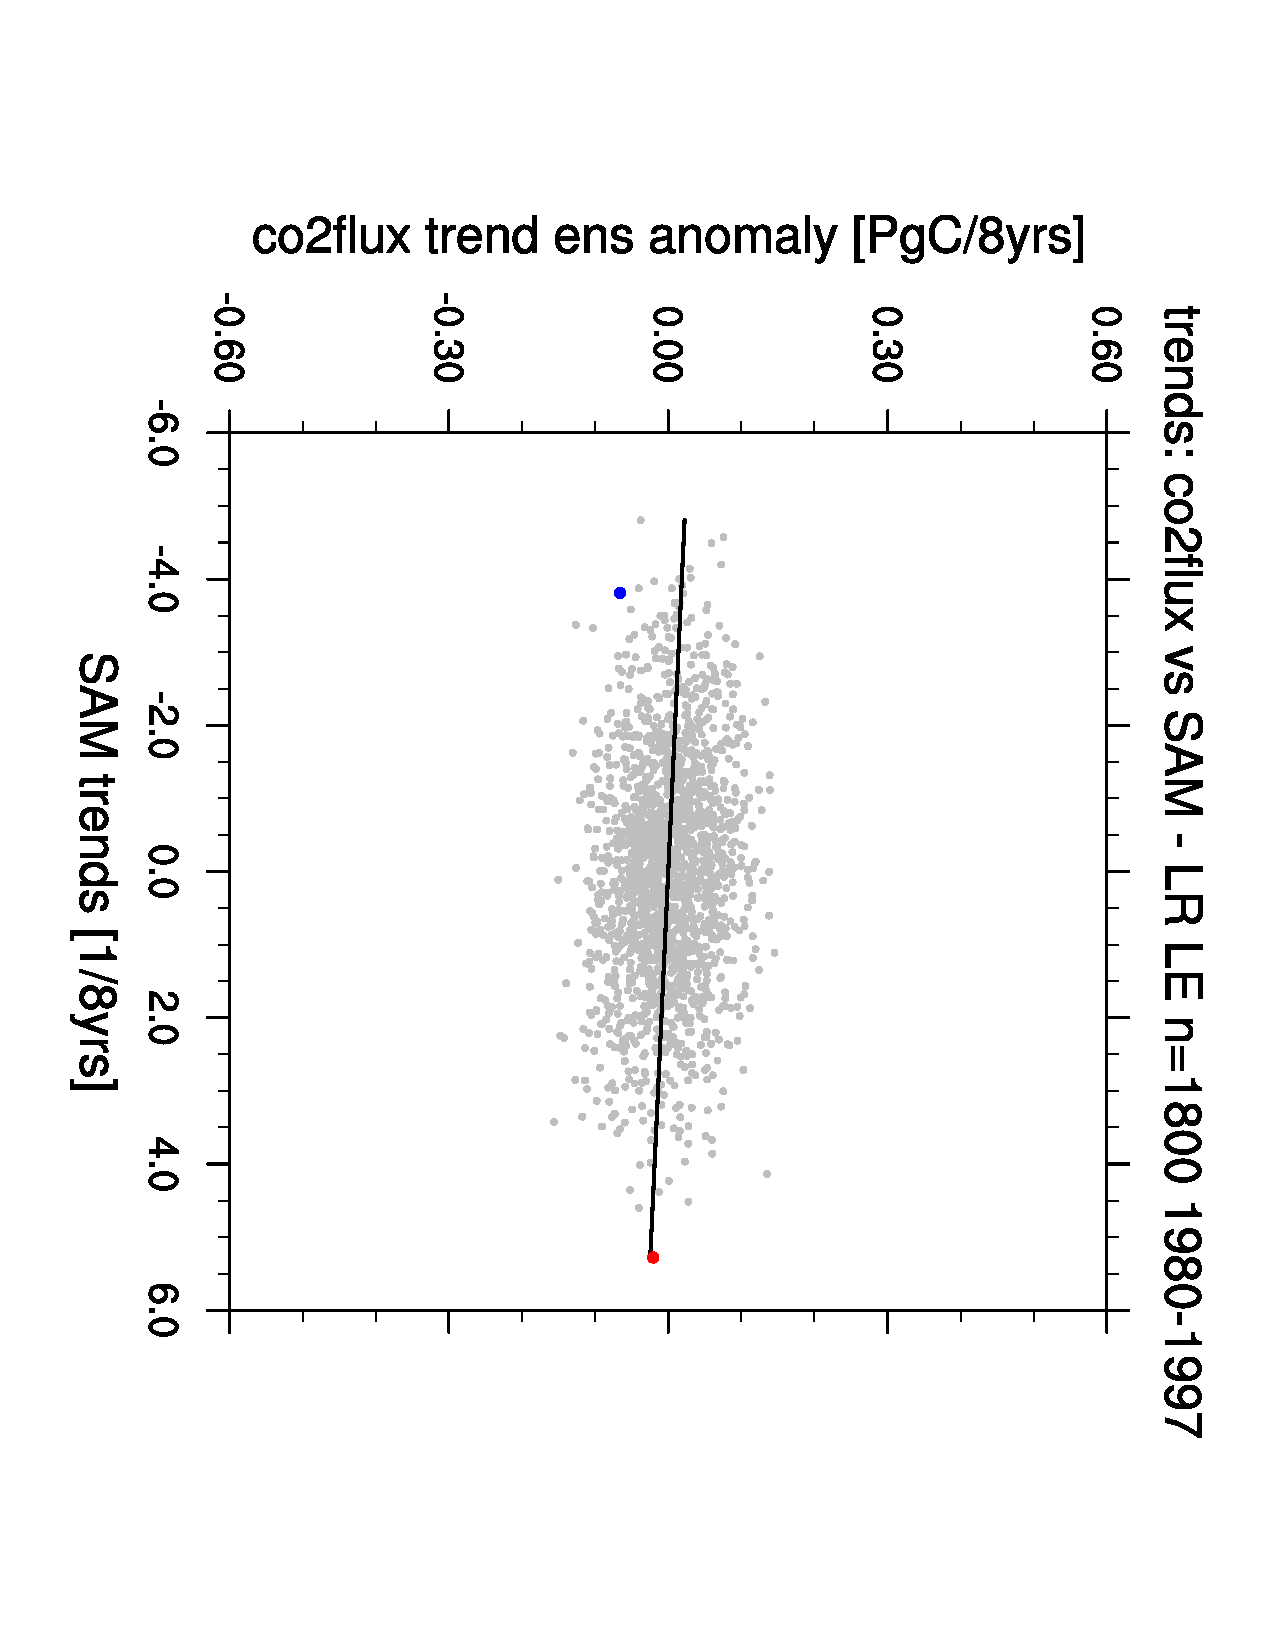
\includegraphics[scale=.38,page=1,angle=90,trim=1.3cm 2.3cm 2.3cm 3cm,clip]{Scatter_trends_bands_ensanom_co2flux_vs_SAM_n1800_1980_1997_trend8_40-49S}
		\vspace{-2mm}
		\caption{Linear trends in the \ac{SAM} as indicator of wind strength vs. sea-air CO$_2$ flux at 50-60$^\circ$S; each data point represents 8-year trends of a single realization normalized for the ensemble mean trend  between 1980 and 2004; the blue dot represents the most negative monotonic CO$_2$ flux trend; the red dot the positive monotonic CO$_2$ flux trend.}
		\label{fig:scatter}
\end{figure}

To qualitatively understand the mechanisms of the Southern Ocean carbon sink I analyze the drivers of CO$_2$ flux on a process level. This chapter covers qualitative CO$_2$ flux changes with respect to the thermal effect, physical circulation and biology. A quantitative analysis of the different drivers for different regions follows in \autoref{ch:pCO2separation}.

The analysis presented here involves 8-year trends for reasons stated in \autoref{sec:choicetrend} but the results of this chapter apply to various multi-year and decadal trends subject to internal variability (not shown).

The spatial trend patterns of different trend periods mostly appear zonally symmetric, therefore the analysis is not separated into the different Southern Ocean sectors, \eg in the Pacific, Indian or Atlantic sector. Also, the atmospheric circulation change in \acs{MPI-ESM} is too symmetric compared to observations \citep{Haumann2014}. Therefore, the description here is carried out in zonal latitudinal bands keeping the unsymmetrical Southern Ocean dynamics in mind \citep{Sallee2010,Talley2013}. Also due to the underestimated Antarctic sea-ice and open-ocean convection in the Ross and Weddell Sea, I restrict my analysis to the Southern Ocean north of 60$^\circ$S, but the decadal CO$_2$ flux trends have a weak signal south of 60$^\circ$S anyway. 



\clearpage

\section{Positive CO$_2$ flux trends}
\label{sec:trends_pos}

Strong positive CO$_2$ flux trends correlate with stronger westerly winds (\autoref{fig:scatter}) \citep{Lovenduski2007}. The difference $\Delta$pCO$_2$ between oceanic pCO$_{2,\text{ocean}}$ and atmospheric partial pressures pCO$_{2,\text{atm}}$ depicts a cleaner signal than CO$_2$ flux (\autoref{fig:pos-co2flux},\ref{fig:pos-dpco2}) and is independent of wind speed and solubility \citep{Lovenduski2015}. pCO$_{2,\text{ocean}}$ rises stronger than pCO$_{2,\text{atm}}$, so CO$_2$ must be driven by changes in the ocean dynamics (\autoref{fig:pos-dpco2}).
The strongest positive signal occurs in the upwelling at 50-60$^\circ$S, a weaker and more patchy signal occurs in the subduction areas north of 50$^\circ$S, whereas changes in most other areas of the Southern Ocean are insignificant (\autoref{fig:pos-dpco2}). 

Westerly winds decrease at 40-50$^\circ$S and increase at 50-60$^\circ$S, which results in a southward shift of westerlies (\autoref{fig:pos-slp}) represented by the positive trend in \acs{SAM} (\autoref{fig:evolution_SAM}). \newline


The response of the thermal effect, upper-ocean overturning circulation and biology are described in \autoref{sec:trends_pos_thermal}, \ref{sec:trends_pos_circulation} and \ref{sec:trends_pos_biology}, respectively.

\begin{figure}[bth]
        \myfloatalign
        \subfloat[CO$_2$ flux trend \text{[kgC m$^{-2}$yr$^{-1}$ /8yrs]}]
        {\label{fig:pos-co2flux}%
        \includegraphics[scale=1.55,trim=13.2cm 18.75cm 4.5cm 6.3cm,clip]{\memberpositive _positive_trend_8_obgc_overview_co2.pdf}} %\quad
        \subfloat[$\Delta$pCO$_2$ trend \text{[ppm/8yrs]}]
        {\label{fig:pos-dpco2}%
         \includegraphics[scale=1.55,trim=13.2cm 15.9cm 4.5cm 9.225cm,clip]{\memberpositive _positive_trend_8_obgc_overview_co2.pdf}} \\
         
         \subfloat[\ac{SLP} and wind trends \text{[hPa/8yrs]}]
        {\label{fig:pos-slp}%
        \includegraphics[scale=1.55,trim=13.2cm 10.2cm 4.5cm 14.9cm,clip]{\memberpositive _positive_trend_8_obgc_overview_co2.pdf}} %\quad
        \subfloat[\ac{SST} trend \text{[$^{\circ}$C/8yrs]}]
        {\label{fig:pos-sst}%
         \includegraphics[scale=1.55,trim=13.18cm 13.05cm 4.5cm 12.075cm,clip]{\memberpositive _positive_trend_8_obgc_overview_co2.pdf}} \\
        \caption{Linear trends during the most positive monotonic 8-year sea-air CO$_2$ flux trend: (a) sea-air CO$_2$ flux, (b) $\Delta$pCO$_2$, (c) \ac{SLP} and wind vectors overlain as arrows and (d) \acf{SST}; hatched areas indicate where trends are outside the 5\% significance level.} \label{fig:pos}
\end{figure}



\clearpage

\subsection{Changes in the thermal effect during positive CO$_2$ flux trends}
\label{sec:trends_pos_thermal}
The solubility of pCO$_{\text{2,ocean}}$ is primarily sensitive to \acf{SST}. Warmer oceans such as the tropical oceans own a lower solubility than cooler high-latitude oceans - a process referred to as the solubility pump of carbon \citep{VolkHoffert1985}. Likewise, CO$_2$-equilibrated waters outgas when warmed and take up CO$_2$ when cooled.

The difference between the partial pressure of CO$_2$ in the ocean (pCO$_{2,\text{ocean}}$) and the atmosphere (pCO$_{2,\text{atm}}$) is the main changing quantity in the CO$_2$ flux formula \citep{Lovenduski2015} (\autoref{eq:HAMOCC}). The separation by \citeauthor{Takahashi1993} [{\color{RoyalBlue}1993}, {\color{RoyalBlue}2002}] gives insights about the direct influence of \ac{SST} (\autoref{sec:takahashi}). The thermal pCO$_2$ trend is driven by changes in \acs{SST} (\autoref{fig:thermal_pos-a}), whereas the non-thermal $\Delta $pCO$_2$ trend approximates all other changes in pCO$_{2,\text{atm}}$, biology, alkalinity, assuming constant \acs{SST} (\autoref{fig:thermal_pos-b}). The thermal pCO$_2$ trend and non-thermal $\Delta$pCO$_2$ trend approximately add up to the trends in pCO$_2$ \citep{landschuetzer2015}. 
The thermal trend follows the \acs{SST} cooling trend (\autoref{fig:pos-sst}) south of 50$^\circ$S towards negative CO$_2$ flux trends, whereas the warming north of 50$^\circ$S favors outgassing. Increased Ekman transport causes this heat divergence in polar regions and a heat convergence at lower latitudes \citep{Hall2002} (\autoref{fig:UOOC_pos}). The non-thermal component strongly increases south of 50$^\circ$S, so overall the pCO$_{2,\text{ocean}}$ increases faster than pCO$_{2,\text{atm}}$ leading to a positive sea-air CO$_2$ flux trend. %This reflects the enhanced outgassing from increased upwelling. 
The non-thermal and thermal trends combined nearly compensate north of 50$^\circ$S but at 50-60$^\circ$S the outgassing dominates (\autoref{fig:pos-dpco2}). The homogenous increase in atmospheric pCO$_{\text{2,atm}}$ accounts for a -12ppm/8yrs in $\Delta$pCO$_2$ (\autoref{fig:pos-dpco2}). %
These changes are stronger in the summer season, especially the non-thermal component because of the stronger summer \acs{SLP} trend (\autoref{fig:pos_summer}, \ref{fig:pos_winter}). 

\begin{figure}[bth]
        \myfloatalign
        \subfloat[pCO$_{\text{2,thermal}}$ trend \text{[ppm/8yrs]}]
        {\label{fig:thermal_pos-a}%
        \includegraphics[scale=1.55,trim=13.2cm 7.3cm 4.5cm 17.785cm,clip]{\memberpositive _positive_trend_8_obgc_overview_co2.pdf}} %\quad
        \subfloat[$\Delta$pCO$_{\text{2,non-thermal}}$ trend \text{[ppm/8yrs]}]
        {\label{fig:thermal_pos-b}%
         \includegraphics[scale=1.55,trim=13.2cm 4.5cm 4.4cm 20.65cm,clip]{\memberpositive _positive_trend_8_obgc_overview_co2.pdf}} \\
        \caption{Linear trends during the most positive monotonic 8-year sea-air CO$_2$ flux trend: (a) pCO$_{2,\text{thermal}}$ and (b) $\Delta$pCO$_{2,\text{non-thermal}}$; hatched areas indicate where trends are outside the 5\% significance level.} \label{fig:thermal_pos}
\end{figure}


\clearpage

\subsection{Changes in ocean circulation during positive CO$_2$ flux trends}
\label{sec:trends_pos_circulation}

Stronger westerly winds intensify the upper-ocean overturning circulation \citep{Lauderdale2013}. Therefore the circulation field advects more \acs{DIC} and alkalinity along its overturning pathway (\autoref{fig:UOOC_pos}). Intensified upwelling of super-saturated waters at 50-60$^\circ$S increase \acs{DIC} and alkalinity concentrations in the euphotic zone (\autoref{fig:ekman_pos-b}). As the pCO$_{\text{2,ocean}}$ sensitivity of \acs{DIC} is larger than for alkalinity, this likely enhances pCO$_{\text{2,ocean}}$, which leads to a positive CO$_2$ flux (for a detailed dicussion see \autoref{ch:pCO2separation}). The stronger winds also increase Ekman northward transport and advects \acs{DIC} and alkalinity further northward (\autoref{fig:ekman_pos-a}). Subduction rates of \ac{AAIW} and \ac{SAMW} formation increase north of 50$^\circ$S, so pCO$_{2,\text{atm}}$-equilibrated waters take additional anthropogenic carbon into the deeper ocean. The southward shift of westerly winds weakens the northern edge of Ekman transport at 30-40$^\circ$S. 

The changes in \ac{MLD} also contribute to the vertical transport of carbon. By deeper mixing in winter, more carbon-rich waters are included into the \acs{MLD}, which then serves as a larger super-saturated reservoir. \acs{MLD} deepens south of 50$^\circ$S and slightly shoals north of 45$^\circ$S, whereas open-ocean convection causes the unrealistic zonal \acs{MLD} averages below 300m south of 60$^\circ$S (\autoref{fig:UOOC_pos}) \citep{Sallee2013,Stoessel2015}. 



\begin{figure}[bth]
        \myfloatalign
        \subfloat[Ekman transport trend \text{[m$^2$ s$^{-1}$/8yrs]}]
        {\label{fig:ekman_pos-a}%
        \includegraphics[scale=1.5,trim=13.1cm 18.75cm 4.5cm 6.38cm,clip]{\memberpositive _positive_trend_8_ekman_overview.pdf}} %\quad
        \subfloat[Ekman pumping trend \text{[m s$^{-1}$/8yrs]}]
        {\label{fig:ekman_pos-b}%
         \includegraphics[scale=1.5,trim=13.25cm 15.9cm 4.1cm 9.2cm,clip]{\memberpositive _positive_trend_8_ekman_overview.pdf}} \\
        \caption{Linear trends during the most positive 8-year sea-air CO$_2$ flux trend: (a) Ekman transport and (b) Ekman pumping; hatched areas indicate where trends are outside the 5\% significance level.} \label{fig:ekman_pos}
\end{figure}


\begin{figure}[hbt]
	\centering
    \captionsetup[subfigure]{labelformat=empty,justification=centering}
	\subfloat[Carbon advection trends \text{[PgC/8yrs]}]{ 
	\includegraphics[scale=0.42,page=2,trim=.3cm 1.7cm 0cm 4.6cm,clip]{UOOC}}
	%\vspace{-5mm}
	\caption{Zonally averaged upper-ocean overturning circulation during the most positive 8-year sea-air CO$_2$ flux trend; black arrows show mean advective carbon transport, red arrows show advective carbon transport trends enforcing the upper-ocean overturning circulation; blue arrows show advective carbon transport trends weakening the upper-ocean overturning circulation; black numbers quantify the trends in advective carbon transport in PgC/8yrs; white lines are isopyncals as in \autoref{fig:UOOC_mean}; grey line is \ac{MLD} in the beginning and the black line MLD in the end of the period.}
	\label{fig:UOOC_pos}
\end{figure}

The upper-ocean overturning circulation response presented here is in-line with idealized wind-change studies \citep{Lauderdale2013}, modeling studies explaining the observed CO$_2$ flux trend in the 1990s \citep{LeQuere2007,Lovenduski2007,Lovenduski2008} as well an inverse modeling study for the 1990s \citep{DeVries2017}.


\clearpage

\subsection{Changes in biology during positive CO$_2$ flux trends}
\label{sec:trends_pos_biology}
The biological pump draws down surface \acf{DIC}, slighty increases alkalinity and is sensitive to changes in circulation (\autoref{fig:deffeyes_processes}). Mixing changes nutrient distributions, when remineralized nutrients from the deep ocean flush into the euphotic zone. Mixing also pulls the standing stock of phytoplankton deeper into the ocean, where less light inhibits growth. Changes in \acs{SST} also directly affect phytoplankton growth (\autoref{sec:HAMOCC}). 

In this subsection, I analyze the 8-year summer (SONDJF) austral summer trends to understand the trends in primary production.\newline
  
Primary production and sea-air CO$_2$ flux show opposing zonally symmetric trend patterns as phytoplankton growth takes up large amounts of surface \acs{DIC}, but only weakly increases alkalinity  and hence lowers pCO$_2$ (\autoref{fig:pos-co2flux}, \ref{fig:summer_trends_pos-intpp}). Primary production declines most pronounced at 50-60$^\circ$S, increases at 40-50$^\circ$S and declines at 30-40$^\circ$S.  The challenge at hand is to find out which changes drive these different responses.
%\paragraph{on intpp not increasing because of more nutrients} different than \citep{Lovenduski2005} 


Internally varying processes change the availability of nutrients. 
The decline in nutrients in the subtropics at 30-40$^\circ$S reduces primary production, but the nutrient availability factor (\autoref{sec:HAMOCC}) slightly increases south of 50$^\circ$S (\autoref{fig:summer_trends_pos-nutrient}).
Previous observational and modeling studies suggest an increase in primary production, because upwelling brings nutrients, especially iron, from the deep-ocean to the iron-limited surface waters \citep{Lovenduski2005,Hauck2013,wang2012,Tagliabue2014}. Additional iron fosters primary production following the iron-hypothesis \citep{Martin1990Nature,Martin1990}, but observational data for iron is still rather sparse to test this for the whole Southern Ocean \citep{Tagliabue2014}. Contrasting \acs{HAMOCC}, many models reproduce this suggested iron-limitation in the Southern Ocean and hence respond with increasing primary production \citep{wang2012,Hauck2013}.  \newline

If the reduction in primary production at 50-60$^\circ$S cannot be explained by changes in nutrients, what else effects primary production blooms?

The combined light \& temperature limitation is primarily driven by temperature after the insulation excels a threshold in cold waters (\autoref{fig:lighttemplimf}). The strong \acs{SST} cooling trend dominates the light \& temperature limitation of primary production. The strong signal in coastal areas as well as Weddell and Ross Sea is attributed to sea-ice changes and open-ocean convection but has minor effects on the primary production and CO$_2$ flux (\autoref{fig:summer_trends_pos-lighttemplim}). 

This northward Ekman transport could also advect phytoplankton northwards to cause the increase in primary production at 40-50$^\circ$S (\autoref{fig:ekman_pos-b}, \ref{fig:summer_trends_pos-intpp}).

The overall decline of primary production in the Southern Ocean under a positive \acs{SAM} trend is also related to mixing. The summer \ac{MLD} has a strong increasing trend at 50-60$^\circ$S, so the mixing deepens (\autoref{fig:summer_trends_pos-zmld}). This is caused by stronger winds (\autoref{fig:pos-slp}) and shown in the average depth of the vertical diffusivity due to wind (\autoref{fig:summer_trends_pos-windmixing}). This deeper mixing in summer then mixes the standing stock of phytoplankton to deeper levels, where they are exposed to less light (\autoref{fig:summer_trends_pos-phydepth}) \citep{Margalef1997}. This theory of a critical depth for phytoplankton blooms was initially proposed by \cite{Sverdrup1953} and requires a stable water column for phytoplankton to initiate blooms. However, this theory is based on turbulent mixing, so the oceanographic \acs{MLD} only serves as a first-order mixing measure for phytoplankton \citep{Franks2014}. Still the signal sustains to phytoplankton depth, where the average phytoplankton depth decreases up to 15m resulting in up to 30\% less light. The lack of monthly output for 3D biogeochemical variables made me use annual averages for phytoplankton, which causes the low significance in \autoref{fig:summer_trends_pos-phydepth}. 

The reverse processes contribute to the increase at 40-50$^\circ$S. Less winds mix less deep and allow phytoplankton to stay more confined to the surface, where they get more light and flourish (\autoref{fig:pos-slp}, \ref{fig:summer_trends_pos-windmixing}, \ref{fig:summer_trends_pos-phydepth}). Also the warming increases the phytoplankton growth rate (\autoref{fig:summer_trends_pos-lighttemplim}).\newline

Summarizing, a multitude of interconnected processes cause the decline in primary production in the Southern Ocean for an increasing \acs{SAM} trend. A clear separation of the magnitude of these interdependent processes is impossible.
 
\begin{figure}[bth]
        \myfloatalign
        \subfloat[INTPP trend \text{[kgCm$^{-2}$yr$^{-1}$/8yrs]}]
        {\label{fig:summer_trends_pos-intpp}%
        \includegraphics[scale=1.55,trim=13.2cm 15.9cm 4.4cm 9.225cm,clip]{\memberpositive _positive_trend_8_obgc_overview_summer.pdf}} %\quad
        \subfloat[Nutrient availability trend \text{[\%/8yrs]}]
        {\label{fig:summer_trends_pos-nutrient}%
         \includegraphics[scale=1.55,trim=13.2cm 13.05cm 4.4cm 12.075cm,clip]{\memberpositive _positive_trend_8_obgc_overview_summer.pdf}} \\
         
         \subfloat[Light- \& temp. limitation trend \text{[\%/8yrs]}]
        {\label{fig:summer_trends_pos-lighttemplim}%
       \includegraphics[scale=1.55,trim=13.2cm 4.5cm 4.4cm 20.65cm,clip]{\memberpositive _positive_trend_8_obgc_overview_summer.pdf}} %\quad
        \subfloat[\acf{MLD} \text{[m/8yrs]}]
        {\label{fig:summer_trends_pos-zmld}%
        \includegraphics[scale=1.55,trim=13.2cm 7.3cm 4.4cm 17.775cm,clip]{\memberpositive _positive_trend_8_obgc_overview_summer.pdf}} \\
         
         \subfloat[Wind mixing depth trend \text{[m/8yrs]}]
        {\label{fig:summer_trends_pos-windmixing}%
        \includegraphics[scale=1.55,trim=13.2cm 15.9cm 4.4cm 9.2cm,clip]{\memberpositive _positive_trend_8_schwerpunkt_mixing_overview.pdf}} %\quad
        \subfloat[Phytoplankton depth trend \text{[m/8yrs]}]
        {\label{fig:summer_trends_pos-phydepth}%
         \includegraphics[scale=1.55,trim=13.2cm 18.7cm 4.4cm 6.38cm,clip]{\memberpositive _positive_trend_8_schwerpunkt_mixing_overview.pdf}} \\
        \caption{Southern Ocean austral summer trends during the most positive 8-year sea-air CO$_2$ flux trend: (a) \acf{INTPP}, (b) nutrient availability factor, (c) surface temperature \& limitation function, (d) \acf{MLD}, (e) average depth of vertical diffusivity due to wind and (f) phytoplankton average depth; hatched areas indicate where trends are outside the 5\% significance level.} \label{fig:summer_trends_pos}
\end{figure}



\clearpage



\section{Negative CO$_2$ flux trends}
\label{sec:trends_neg}

Disclaimer: Generally, in this analysis the direction of trends reverse for weakening and northward-shifting westerlies, which leads to an overall negative sea-air CO$_2$ flux trend. Additionally, now the prescribed atmospheric pCO$_{\text{2,atm}}$ forcing promotes a steady negative background sea-air CO$_2$ flux trend.\newline

A strong negative sea-air CO$_2$ flux trends correlates with weaker westerly winds (\autoref{fig:neg-co2flux}, \ref{fig:neg-slp}). The strongest negative signal $\Delta$pCO$_2$ occurs in the upwelling area at 50-60$^\circ$S. Changes in most other areas of the Southern Ocean are insignificant (\autoref{fig:neg-dpco2}). 

%Westerly winds decrease at 40-60$^\circ$S, which results in a northward shift of westerlies (\autoref{fig:pco2_pos}) represented by the negative trend in \acs{SAM} (\autoref{fig:evolution_SAM}).

%The strengthening of the Southern Ocean carbon sink under the context of intensified westerly winds leads me to a hypothesis (fig. \autoref{fig:schematics_pos}):
%Weaker winds at 50-60$^\circ$S slow down the upper-ocean overturning circulation and increase primary production due to a more stable water column. [really unsure about this hypothesis part - I dont discover anything new but want to explain the process with a figure ahead]
The response in the thermal effect, upper-ocean overturning circulation and biology are described in \autoref{sec:trends_neg_thermal}, \ref{sec:trends_neg_circulation} and \ref{sec:trends_neg_biology}, respectively.

\begin{figure}[bth]
        \myfloatalign
        \subfloat[CO$_2$ flux trend \text{[kgC m$^{-2}$yr$^{-1}$ /8yrs]}]
        {\label{fig:neg-co2flux}%
        \includegraphics[scale=1.55,trim=13.2cm 18.75cm 4.5cm 6.3cm,clip]{\membernegative _positive_trend_8_obgc_overview_co2.pdf}} %\quad
        \subfloat[$\Delta$pCO$_2$ trend \text{[ppm/8yrs]}]
        {\label{fig:neg-dpco2}%
         \includegraphics[scale=1.55,trim=13.2cm 15.9cm 4.5cm 9.225cm,clip]{\membernegative _positive_trend_8_obgc_overview_co2.pdf}} \\
         
         \subfloat[\ac{SLP} and wind trends \text{[hPa/8yrs]}]
        {\label{fig:neg-slp}%
        \includegraphics[scale=1.55,trim=13.2cm 10.2cm 4.5cm 14.9cm,clip]{\membernegative _positive_trend_8_obgc_overview_co2.pdf}} %\quad
        \subfloat[\ac{SST} trend \text{[$^{\circ}$C/8yrs]}]
        {\label{fig:neg-sst}%
         \includegraphics[scale=1.55,trim=13.18cm 13.05cm 4.5cm 12.075cm,clip]{\membernegative _positive_trend_8_obgc_overview_co2.pdf}} \\
        \caption{Linear trends during the most negative monotonic 8-year air-sea CO$_2$ flux trend: (a) sea-air CO$_2$ flux, (b) $\Delta$pCO$_2$, (c) \ac{SLP} and wind vectors overlain as arrows and (d) \acf{SST}; hatched areas indicate where trends are outside the 5\% significance level.} \label{fig:neg}
\end{figure}



\clearpage

\subsection{Changes in the thermal effect during negative CO$_2$ flux trends}
\label{sec:trends_neg_thermal}

The \ac{SST} warming trend (\autoref{fig:neg-sst}) drives the thermal trend south of 50$^\circ$S towards a positive pCO$_{2,\text{ocean}}$ trend, whereas the cooling north of 50$^\circ$S results in a pCO$_{2,\text{ocean}}$ decline (\autoref{fig:thermal_neg-a}). These \acs{SST} changes are caused by less Ekman transport and lead to a heat convergence in the polar region and a heat divergence in the subtropics \citep{Hall2002}. The non-thermal trend has a strong negative signal south of 50$^\circ$S and a slightly positive north of 50$^\circ$S (\autoref{fig:thermal_neg-b}). The increase in atmospheric pCO$_{\text{2,atm}}$ accounts for a -14ppm/8yrs. The non-thermal and thermal trends combined nearly compensates north of 50$^\circ$S, but the non-thermal component dominates at 50-60$^\circ$S (\autoref{fig:neg-dpco2}). 

These changes are stronger in the summer season, especially the non-thermal component, because of the stronger \acs{SLP} winter trends (\autoref{fig:neg_summer}, \ref{fig:neg_winter}). 
 
\begin{figure}[bth]
        \myfloatalign
        \subfloat[pCO$_{\text{2,thermal}}$ trend \text{[ppm/8yrs]}]
        {\label{fig:thermal_neg-a}%
        \includegraphics[scale=1.55,trim=13.2cm 7.3cm 4.5cm 17.785cm,clip]{\membernegative _positive_trend_8_obgc_overview_co2.pdf}} %\quad
        \subfloat[$\Delta$pCO$_{\text{2,non-thermal}}$ trend \text{[ppm/8yrs]}]
        {\label{fig:thermal_neg-b}%
         \includegraphics[scale=1.55,trim=13.2cm 4.5cm 4.4cm 20.65cm,clip]{\membernegative _positive_trend_8_obgc_overview_co2.pdf}} \\
        \caption{Linear trends during the most negative monotonic 8-year sea-air CO$_2$ flux trend: (a) pCO$_{2,\text{thermal}}$ and (b) $\Delta$pCO$_{2,\text{non-thermal}}$; hatched areas indicate where trends are outside the 5\% significance level.} \label{fig:thermal_neg}
\end{figure}




\clearpage

\subsection{Changes in ocean circulation during negative CO$_2$ flux trends}
\label{sec:trends_neg_circulation}

Weaker westerly winds weaken the upper-ocean overturning circulation \citep{Lauderdale2013}, so the circulation field advects less \acs{DIC} and alkalinity along its overturning pathway (\autoref{fig:UOOC_neg}). Less upwelling at 50-60$^\circ$S decreases \acs{DIC} and alkalinity concentrations in the euphotic zone (\autoref{fig:ekman_neg-pumping}). Weaker winds also decrease Ekman northward transport and reduce northward advection of \acs{DIC} and alkalinity (\autoref{fig:ekman_neg-transport}). North of 50$^\circ$S subduction rates of \acs{AAIW} and \acs{SAMW} formation decrease, which could also be a sign of a northward-shift in upwelling. The \acs{MLD} shoals south of 50$^\circ$S and slightly deepens north of 45$^\circ$S (\autoref{fig:UOOC_neg}). 


\begin{figure}[hbt]
        \myfloatalign
        \subfloat[Ekman transport trend \text{[m$^2$ s$^{-1}$/8yrs]}]
        {\label{fig:ekman_neg-transport}%
        \includegraphics[scale=1.5,trim=13.1cm 18.75cm 4.5cm 6.38cm,clip]{\membernegative _positive_trend_8_ekman_overview.pdf}} %\quad
        \subfloat[Ekman pumping trend \text{[m s$^{-1}$/8yrs]}]
        {\label{fig:ekman_neg-pumping}%
         \includegraphics[scale=1.5,trim=13.25cm 15.9cm 4.1cm 9.2cm,clip]{\membernegative _positive_trend_8_ekman_overview.pdf}} \\
        \caption{Linear trends during the most negative 8-years sea-air CO$_2$ flux trend: (a) Ekman transport and (b) Ekman pumping; hatched areas indicate where trends are outside the 5\% significance level.} \label{fig:ekman_neg}
\end{figure}


\begin{figure}[hbt]
	\centering
	\captionsetup[subfigure]{labelformat=empty,justification=centering}
	\subfloat[Carbon advection trends \text{[PgC/8yrs]}]{ 
	\includegraphics[scale=0.42,page=3,trim=.3cm 1.7cm 0cm 4.cm,clip]{UOOC}}
	%\includegraphics[scale=0.5,page=3,trim=1.4cm 1.7cm 0cm 4.6cm,clip]{UOOC}
	%\vspace{-10mm}
	\caption{Zonally averaged upper-ocean overturning circulation during the most negative 8-year sea-air CO$_2$ flux trend; black arrows show mean advective carbon transport, red arrows show advective carbon transport trends enforcing the upper-ocean overturning circulation; blue arrows show advective carbon transport trends weakening the upper-ocean overturning circulation; black numbers show the trends in advective carbon transport in PgC/8yrs; white lines are isopyncals as in \autoref{fig:UOOC_mean}; grey line is \ac{MLD} in the beginning and the black line MLD in the end of the period.}%; black arrows show mean advective carbon transport, red arrows show advective carbon transport trend over 8 years; white lines are isopyncals separating Sub-Antarctic Mode Water (SAMW), Antarctic Intermediate Water (AAIW), Circumpolar Deep Water (CDW) and Antarctic Bottom Water (AABW)}
	\label{fig:UOOC_neg}
\end{figure}


This upper-ocean overturning circulation response agrees with idealized wind-change studies \citep{Lauderdale2013}. The inverse modeling study reports a decline from the 2000s towards the previous decade \citep{DeVries2017}, which could be related to changes in wind. However, \cite{landschuetzer2015} did not report a strong negative trend for the strength of observed westerly winds, but a pattern change in \acs{SLP} in the 2000s became more zonally asymmetric. On the contrary, depending on the starting year of the trend period, the \acs{SAM} index slightly weakened in the early 2000s \citep{Marshall2003,Lovenduski2015}.


\clearpage

\subsection{Changes in biology during negative CO$_2$ flux trends}
\label{sec:trends_neg_biology}

%The biological pump draws down surface DIC and sensitive to changes in circulation (see section \autoref{sec:HAMOCC}). In this subsection, I analyze the 8-year summer (SONDJF) austral summer trends. 
  
Primary production and CO$_2$ flux show opposing zonally symmetric trend patterns (\autoref{fig:neg-co2flux}, \ref{fig:summer_trends_neg-intpp}). The patchy trend patterns of primary production increase  most dominant at 50-60$^\circ$S, decrease at 40-50$^\circ$S and increase at 30-40$^\circ$S. %Which changes drive these different responses?
%\paragraph{on intpp not increasing because of more nutrients} different than \citep{Lovenduski2005} 

%Internally varying processes change the availability of nutrients. 
The additional supply of nutrients in the subtropics at 30-40$^\circ$S fosters primary production, because the northward-shift in upwelling flushes nutrients from the deep into the nutrient-depleted subtropical gyre region. South of 45$^\circ$S the nutrient availability hardly changes and decreases (\autoref{fig:summer_trends_neg-nutrient}). 
Previous observational and modeling studies suggest decreasing in primary production because less upwelling brings less nutrients, especially iron, from the deep-ocean to the surface \citep{Hauck2013,Tagliabue2014}. But the Southern Ocean in \acs{HAMOCC} is nitrate limited, so the slight reduction in nutrients rather originates in the increased nutrient consumption due to primary production.  %\newline

%If the reduction in primary production at 50-60$^\circ$S cannot be explained by changes in nutrients, what else effects primary production blooms?

The \acs{SST} trends enhance primary production at 50-60$^\circ$S and lower primary production north of 50$^\circ$S (\autoref{fig:summer_trends_neg-lighttemplim}). %The strong light \& temperature limitation signal in coastal areas as well as Weddell and Ross Sea is attributed to sea-ice changes and open-ocean convection, but has minor effects on the primary production and CO$_2$ flux (fig. \autoref{fig:summer_trends_neg}d). 

The weakened northward Ekman transport also keeps the standing stock more southwards and causes the increase in primary production at 50-60$^\circ$S and the shifted decrease at 40-50$^\circ$S (\autoref{fig:ekman_neg}). 

Weaker winds mix the ocean less deep and thereby keeps the standing stock of phytoplankton in more light-flooded levels at 50-60$^\circ$S (\autoref{fig:summer_trends_neg-windmixing}).
The reverse process contributes to the decrease at 40-50$^\circ$S.\newline

Overall, primary production decreases for weaker and northward-shifting winds.
%Summarizing, a multitude of interconnected processes caused the increase in primary production in the Southern Ocean for a decreasing SAM trend. A clear separation of the magnitude of the different effects is impossible.
 


\begin{figure}[bth]
        \myfloatalign
        \subfloat[INTPP trend \text{[kgCm$^{-2}$yr$^{-1}$/8yrs]}]
        {\label{fig:summer_trends_neg-intpp}%
        \includegraphics[scale=1.55,trim=13.2cm 15.9cm 4.4cm 9.225cm,clip]{\membernegative _positive_trend_8_obgc_overview_summer.pdf}} %\quad
        \subfloat[Nutrient availability trend \text{[\%/8yrs]}]
        {\label{fig:summer_trends_neg-nutrient}%
         \includegraphics[scale=1.55,trim=13.2cm 13.05cm 4.4cm 12.075cm,clip]{\membernegative _positive_trend_8_obgc_overview_summer.pdf}} \\
         
         \subfloat[Light- \& temp. limitation trend \text{[\%/8yrs]}]
        {\label{fig:summer_trends_neg-lighttemplim}%
       \includegraphics[scale=1.55,trim=13.2cm 4.5cm 4.4cm 20.65cm,clip]{\membernegative _positive_trend_8_obgc_overview_summer.pdf}} %\quad
        \subfloat[\acf{MLD} \text{[m/8yrs]}]
        {\label{fig:summer_trends_neg-zmld}%
        \includegraphics[scale=1.55,trim=13.2cm 7.3cm 4.4cm 17.775cm,clip]{\membernegative _positive_trend_8_obgc_overview_summer.pdf}} \\
         
         \subfloat[Wind mixing depth trend \text{[m/8yrs]}]
        {\label{fig:summer_trends_neg-windmixing}%
        \includegraphics[scale=1.55,trim=13.2cm 15.9cm 4.4cm 9.2cm,clip]{\membernegative _positive_trend_8_schwerpunkt_mixing_overview.pdf}} %\quad
        \subfloat[Phytoplankton depth trend \text{[m/8yrs]}]
        {\label{fig:summer_trends_neg-phydepth}%
         \includegraphics[scale=1.55,trim=13.2cm 18.7cm 4.4cm 6.38cm,clip]{\membernegative _positive_trend_8_schwerpunkt_mixing_overview.pdf}} \\
        \caption{Southern Ocean austral summer trends during the most negative sea-air 8-year CO$_2$ flux trend: (a) vertically integrated primary production (INTPP), (b) nutrient availability factor, (c) surface temperature \& limitation function, (d) \acf{MLD}, (e) average depth of vertical diffusivity due to wind and (f) phytoplankton average depth; hatched areas indicate where trends are outside the 5\% significance level.} \label{fig:summer_trends_neg}
\end{figure}
%************************************************
\chapter{Discussion}\label{ch:discussion} % $\mathbb{ZNR}$
%************************************************

%\section{Some Formulas}
\citep{landschuetzer2015} \\
\citep{LeQuere2007}\\
\citep{Lovenduski2005}\\ 
\citep{Lovenduski2007}\\
\citep{Lovenduski2008}\\
\citep{Hauck2013}\\
\citep{wang2012}\\
\vspace{3cm}

\citep{Lovenduski2005}: how is model different, how are results different
\begin{enumerate}
\item our MLD responds differently than Lovenduski2005 Fig.2 schematic illustration
\item increase in SAM --> increase in chlorophyll south of PF/45°S because of iron supply from below (we have phy-decrease)
\item increase in SAM --> reduction in chlorophyll north of PF/45°S because of increased ZMLD (we have a slight phy-increase)
\item BUT we dont have iron limitation in SO, so this study can be used as a direct physical effect of stronger winds on primary production excluding nutrient supply changes
\end{enumerate} 

\citep{Hauck2013}: stronger winds, increased upwelling, more iron supply, higher primary production

\citep{wang2012}: 
\begin{enumerate}
\item forced model, 25yr trends, so rather climate change impact than decadal variability
\item some regions: more upwelling, more iron, more primary production 
\item I dont get the clear storyline of the whole paper
\end{enumerate}

Limitations of HAMOCC vs obs/other models:
\begin{enumerate}
\item too early and enhanced Southern Ocean seasonal cycle \citep{Nevison2016}
\item not eddy resolving, has impacts \citep{Marshall2012,Stoessel2015}
\item location of polar jets in ECHAM %[I remember this from a group meeting, but didnt check so far]
\item basically no nutrient limitation in SO? - other models and observations disagree
\item other observation studies use sparse for pCO2 or proxy (satelite chl-a)
\item MPIOM performance on circulation patterns and water masses in SO %(Yohei mentioned Anne M. could know this)
\item only one phytoplankton type in HAMOCC? - more variety of plankton species might be able to adapt to depth? or is this too unrealistic for a global model such as HAMOCC?
\item MPI-ESM zmld performance in SO \citep{Sallee2013}
\end{enumerate} 
%************************************************
%\chapter{Summary and conclusions} % $\mathbb{ZNR}$
\chapter{Summary, Conclusions and Outlook} \label{ch:conclusions}% $\mathbb{ZNR}$
%************************************************

%zusammenfassen und heftig verlinken und zitieren
%\paragraph{Summary} %and internal variability value $\pm$X; make sure research questions are answered}
% explicit revisiting research questions
To assess decadal internal variability of the Southern Ocean sea-air CO$_2$ flux, I analyzed the large ensemble of 100 \acl{MPI-ESM} simulations (\acs{MPI-ESM LE}) in the historical period from 1980 to 2004, for which the observational sea-air CO$_2$ flux product \acf{SOM-FFN} is available. I summarize this thesis by revisiting the research questions posed in the introduction.\newline %and conclude

\textit{What is the modeled internal variability of the Southern Ocean carbon sink?}\\

I estimate the modeled decadal internal variability to $\sigma_{DIV}\sim\pm0.19$ PgC/yr/decade (\autoref{fig:evolution_southern_ocean_carbon_sink}, \ref{fig:SOCS_temporal_gaussian-a}). Compared to the 1980-2004 mean sea-air CO$_2$ flux south of 35$^\circ$S of $\sim-1.15$ PgC/yr, decadal internal variability $\sigma_{DIV}$ amounts to $\sim12\%$. In addition, internal variability dominates over the forced signal of $\sim-0.14$ PgC/yr/decade and is hence crucial in evaluating changes in the Southern Ocean carbon sink. %This magnitude suggests that internal variability might be able to oppress the anthropogenic climate change signal of two decades in the Southern Ocean, which is in-line with the emergence of the anthropogenic climate change signal in the certain areas Southern Ocean carbon sink in \acs{CESM} \acs{LE} after 20 years \citep{McKinley2016}. 

The area at 50-60$^\circ$S holds the largest decadal variability (\autoref{fig:SOCS_ensmean_ensstd-b}) and dominates the overall Southern Ocean CO$_2$ flux trend (\autoref{ch:trends}). \acs{MPI-ESM LE} contains decadal trends of sea-air CO$_2$ flux of the same magnitude of $\sim+0.5$ PgC/yr/decade and $\sim-0.7$ PgC/yr/decade but less monotonic behavior as suggested by observations \citep{landschuetzer2015} (\autoref{fig:heatmap}).  
The same monotonic behavior as observations is found in 8-year trends of $\sim+0.5$ PgC/yr/8yrs and $\sim-0.6$ PgC/yr/8yrs (\autoref{fig:evolution_southern_ocean_carbon_sink}). The underlying source and responses in the carbon sink are analogous on decadal and multi-year time-scale. \newline

\textit{What are the sources of this internal variability?}\\

I investigate the sources of internal variability as the origins which trigger internally varying responses of CO$_2$ flux from thermal, physical and biological processes. The major source is the variability in strength and position of westerly winds. I find two distinct wind-driven regimes in the area of at 50-60$^\circ$S with the largest internal variability of sea-air CO$_2$ flux (\autoref{fig:scatter}): 

On the one hand stronger and southward-shifting westerly winds associated with a positive trend in the \acf{SAM} reduce the Southern Ocean carbon sink. On the other hand weakening and northward-shifting westerly winds lead to an increase in the Southern Ocean carbon sink.\newline

\textit{What are the contributions of different processes to multi-year trends in sea-air CO$_2$ flux in the Southern Ocean?}\\

%atm sst circ bio
The increasing atmospheric pCO$_{\text{2,atm}}$ drives the sea-air CO$_2$ flux trends towards a more CO$_2$ uptake state, whereas oceanic pCO$_{\text{2,ocean}}$ is susceptible to internally varying processes:

For intensifying and southward shifting westerly winds, \acf{SST} cooling drives pCO$_{\text{2,ocean}}$ decrease (\autoref{sec:trends_pos_thermal}). Cooling and deeper wind-mixing reduce primary production, which increases pCO$_{\text{2,ocean}}$ (\autoref{sec:trends_pos_biology}). These responses are dominated by a process that cannot be accounted for directly and is likely the increased upper-ocean overturning circulation, which enhances outgas-sing of deep waters and overall weakens the Southern Ocean carbon sink (summarizing \autoref{fig:schematics_pos}). %(\autoref{ch:pCO2separation}). 

Vice versa, for weaker and northward-shifting westerly winds the trends in the different processes reverse. Decreasing upwelling and increased primary production result in little oceanic pCO$_{\text{2,ocean}}$ decrease, and only combined with the strong atmospheric pCO$_{\text{2,atm}}$ increase the Southern Ocean carbon sink increases (summarizing \autoref{fig:schematics_neg}).\newline %[how deep should the summary of processes go? now its shallow! should I talk about thermal, bio and circulation explicitly - I already evaluate the processes in the chapter right before!]\newline

\vspace{.5cm}

%\paragraph{Comparability to observations}
\label{sec:conlcusions}
What can be learned from this large ensemble simulation about the Southern Ocean carbon sink? 

While \acs{MPI-ESM LE} aims to capture model spread due to internal variability and not reproduce CO$_2$ flux trends suggested by observations in the first place, I find that perturbed initial conditions large ensemble simulations are capable of capturing decadal internal variations similar to observations; even though other ensembles such as from \acs{GFDL} or \acs{NCAR} do not and this only applies for the most extreme decadal trends in \acs{MPI-ESM LE}.

Forcing \acs{MPI-ESM} with historical CO$_2$ emissions instead of prescribed pCO$_{\text{2,atm}}$ increases internal variability of the global carbon sink by 25\% \citep{Ilyina2013}. Therefore, in an emission-driven \acs{ESM} configuration with interactive carbon cycle, the internal variability of the Southern Ocean carbon sink could be an even higher $\sigma_{DIV}$. 

The strong trends discussed in this thesis originate in strong changes of the position and strength of Southern hemisphere westerly winds and effect of those on ocean circulation. However, the parametrized eddies in \acs{MPI-ESM LE} might allow deeper mixing to sustain on longer time-scales than the seasonal timescale at which the eddies would counteract those trends \citep{Thompson2011}. The impact of eddies on the carbon cycle in high-resolution simulations, especially in the Southern Ocean, is under current research \citep{Ito2010,Dufour2013,Gnanadesikan2015,Meredith2016}. Only a variable definition of isopyncal thickness diffusion could parametrize the expected eddy response from high-resolution simulations \citep{Gent2011}. \cite{Lovenduski2013} reproduce these increasing eddy fluxes and the response to the carbon cycle, but the general challenge of differing ocean circulation patterns remains and makes a comparison between a high-resolution resolved eddies and low-resolution parametrized eddies impossible \citep{Bryan2014}. %transition to outlook
A future possible high-resolution perturbed initial conditions ensemble simulations would give a more realistic representation of internal variability.\newline



%\paragraph{Outlook: observational focus on Southern Ocean}  
% new obs, and missing model variability
This thesis suggests that even though decadal variations are captured, decadal trends as in \cite{landschuetzer2015} are rare and raise the question whether biogeochemical processes are missing or implemented in overestimated robustness. From an observational perspective, the historically under-sampled Southern Ocean now got equipped with ARGO floats, including 200 floats with biogeochemical sensors. This permits accurate in-situ measurements for the first time during austral winter months and even under ice making it possible to build and constrain biogeochemical models to primary production in melt ponds or under thinning sea-ice. Most models lack this potentially additional variable contribution to the oceanic carbon sink \citep{Long2015,Williams2017,Horvat2017}.

%on modeling physical challenges
The Southern Ocean water-column is very susceptible to density changes. Modeling the Southern Ocean where different water masses converge, faces long-standing challenges with water-column stability. Open-ocean convection appears in models although not observed for decades \citep{deLavergne2014,Stoessel2015}. Sea-ice is underestimated in \acs{MPI-ESM} \citep{Jungclaus2013,Notz2013}. Additional freshwater input from icebergs would stratify the high-latitude Southern Ocean and thereby hinder open-ocean convection and excessive winter mixing \citep{Sallee2013,Stoessel2015}. A higher-resolution atmosphere would introduce oceanic counter gyres in the Weddell and Ross Sea, which push the sea-ice edge to more realistic and northern extent \citep{Stoessel2015}. Introducing these developments to \acs{MPI-ESM} would benefit the biogeochemical representation in \acs{HAMOCC}.\newline

%, there is a need for an increasing amount of measurements to understand the Southern Ocean dynamics and biogeochemical properties. The recent ARGO data and the newly deployed biogeochemical floats currently advance the basis for understanding in the Southern Ocean. %Elevating  numbers of in-situ measurements help to overcome the current challenges in Southern Ocean modeling \citep{Sallee2013,Sallee2013a,Jungclaus2013,deLavergne2014,Haumann2014,Stoessel2015,Haumann2016}.   
%no strong finnish :(
\label{sec:outlook}
%\paragraph{Outlook: large ensemble variability modeling}
The history of large ensemble simulations with perturbed initial conditions is fairly recent. The attempt to study internal variability with \acs{MPI-ESM LE} gives first insights into internal variability from many realizations of simulations. A further interesting project would be the comparison of different perturbed initial conditions large ensembles based on different models, \ie comparing \acs{CESM} \acs{LE}, \acs{GFDL} \acs{LE} and \acs{MPI-ESM LE}. 

All in all it becomes increasingly important to understand internal varying processes in our climate system in the case of global CO$_2$ emission reductions, when CO$_2$ reduction efforts are tracked by measurements and evaluated by scientists and politicians \citep{Hawkins2009,McKinley2016,Lovenduski2016,Marotzke2017}.\newline

%geiler schlusssatz

%\include{multiToC} % <--- just debug stuff, ignore for your documents
% ********************************************************************
% Backmatter
%*******************************************************
\appendix
%\renewcommand{\thechapter}{\alph{chapter}}
\cleardoublepage
%\part{Appendix}
%********************************************************************
% Appendix
%*******************************************************
% If problems with the headers: get headings in appendix etc. right
%\markboth{\spacedlowsmallcaps{Appendix}}{\spacedlowsmallcaps{Appendix}}
\chapter{Appendix}
Lorem ipsum at nusquam appellantur his, ut eos erant homero
concludaturque. Albucius appellantur deterruisset id eam, vivendum
partiendo dissentiet ei ius. Vis melius facilisis ea, sea id convenire
referrentur, takimata adolescens ex duo. Ei harum argumentum per. Eam
vidit exerci appetere ad, ut vel zzril intellegam interpretaris.
\graffito{More dummy text.}

%Errem omnium ea per, pro congue populo ornatus cu, ex qui dicant
%nemore melius. No pri diam iriure euismod. Graecis eleifend
%appellantur quo id. Id corpora inimicus nam, facer nonummy ne pro,
%kasd repudiandae ei mei. Mea menandri mediocrem dissentiet cu, ex
%nominati imperdiet nec, sea odio duis vocent ei. Tempor everti
%appareat cu ius, ridens audiam an qui, aliquid admodum conceptam ne
%qui. Vis ea melius nostrum, mel alienum euripidis eu.

\section{Statistics of Southern Ocean carbon sink}
\begin{figure}[h]
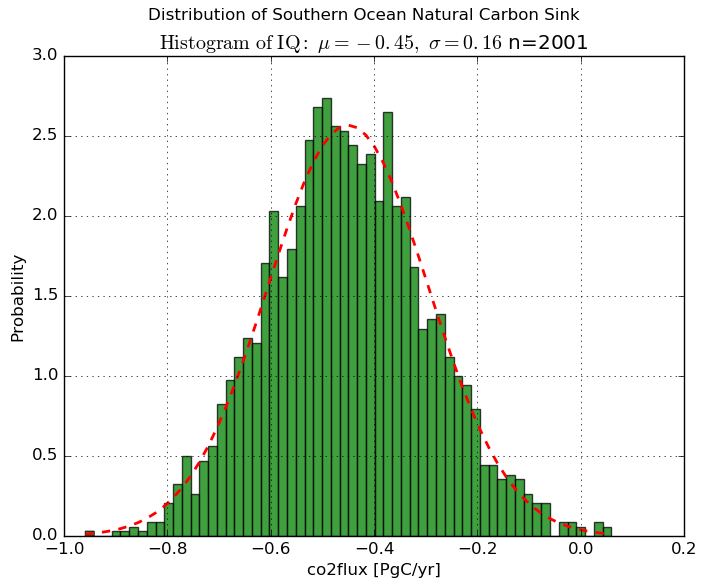
\includegraphics[scale=.4]{gfx/SOCS_temporal_gaussian.png} % from gfx folder
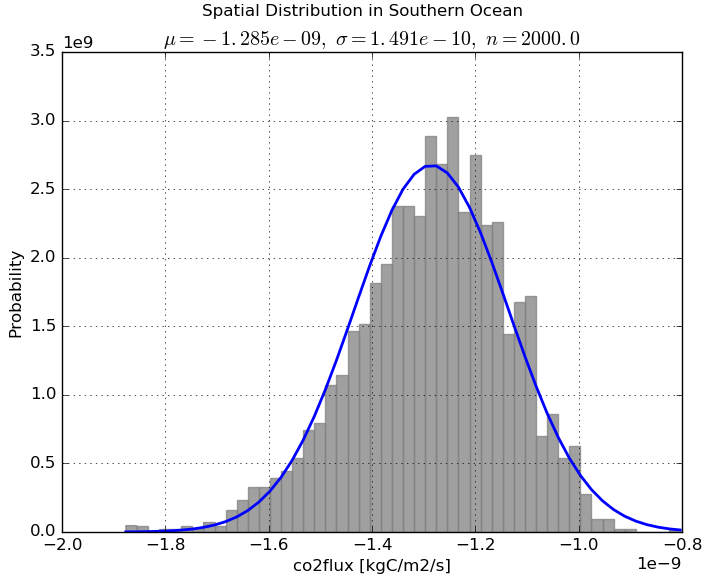
\includegraphics[scale=.4]{gfx/SOCS_spatial_gaussian.png} % from gfx folder
\caption{Southern Ocean carbon sink: yearmean fieldsum 35-90S (left) and yearmean in a random grid cell (right)}
\label{fig:SOCS_temporal_gaussian}
\end{figure}



\cleardoublepage%*******************************************************
% List of Figures and of the Tables
%*******************************************************
\clearpage
\begingroup 
    \let\clearpage\relax
    \let\cleardoublepage\relax
    \let\cleardoublepage\relax
    %*******************************************************
    % List of Figures
    %*******************************************************    
	\section{\listfigurename}     
    %\phantomsection 
    \refstepcounter{dummy}
    %\addcontentsline{toc}{section}{\listfigurename}
 %   \pdfbookmark[1]{\listfigurename}{lof}
    \listoffigures

    \vspace{8ex}

    %*******************************************************
    % List of Tables
    %*******************************************************
%	\section{\listtablename}     
    %\phantomsection 
 %   \refstepcounter{dummy}
    %\addcontentsline{toc}{section}{\listtablename}
  %  \pdfbookmark[1]{\listtablename}{lot}
  %  \listoftables
        
 %   \vspace{8ex}
%   \newpage
    
    %*******************************************************
    % List of Listings
    %*******************************************************      
%	\section{\lstlistlistingname}     
      %\phantomsection 
 %   \refstepcounter{dummy}
    %\addcontentsline{toc}{section}{\lstlistlistingname}
    %\addcontentsline{toc}{chapter}{\lstlistlistingname}
 %   \pdfbookmark[1]{\lstlistlistingname}{lol}
    %\lstlistoflistings 

 %   \vspace{8ex}
       
    %*******************************************************
    % Acronyms
    %*******************************************************
    %\phantomsection 
%    \refstepcounter{dummy}
    %\pdfbookmark[1]{Acronyms}{acronyms}
    %\markboth{\spacedlowsmallcaps{Acronyms}}{\spacedlowsmallcaps{Acronyms}}
    %\chapter*{Acronyms}
    %\begin{acronym}[UMLX]
    %    \acro{DRY}{Don't Repeat Yourself}
    %    \acro{API}{Application Programming Interface}
    %    \acro{UML}{Unified Modeling Language}
    %\end{acronym}                     
\endgroup


%********************************************************************
% Other Stuff in the Back
%*******************************************************
\cleardoublepage%********************************************************************
% Bibliography
%*******************************************************
% work-around to have small caps also here in the headline
\manualmark
\markboth{\spacedlowsmallcaps{\bibname}}{\spacedlowsmallcaps{\bibname}} % work-around to have small caps also
%\phantomsection 
\refstepcounter{dummy}
\addtocontents{toc}{\protect\vspace{\beforebibskip}} % to have the bib a bit from the rest in the toc
\addcontentsline{toc}{chapter}{\tocEntry{\bibname}}
\label{app:bibliography}
%\bibliographystyle{abbrvnat}
\printbibliography
\cleardoublepage%*******************************************************
% Acknowledgments
%*******************************************************
\pdfbookmark[1]{Acknowledgments}{acknowledgments}

%\begin{flushright}{\slshape    
%    We have seen that computer programming is an art, \\ 
%    because it applies accumulated knowledge to the world, \\ 
%    because it requires skill and ingenuity, and especially \\
%    because it produces objects of beauty.} \\ \medskip
%    --- \defcitealias{knuth:1974}{Donald E. Knuth}\citetalias{knuth:1974} \citep{knuth:1974}
%\end{flushright}

%\let\clearpage\relax
%\let\cleardoublepage\relax
%\let\cleardoublepage\relax
\chapter*{Acknowledgments}

Writing this thesis was an incredible journey of personal learning and failures, which I could not have accomplished without the help of my environment.\newline

I thank my supervisors Tatiana Ilyina for setting the foundations of this thesis and guidance in contents, and Norbert Frank for external feedback and encouraging me to apply to an external research center like \acf{MPI}.\newline

I enjoyed my visit to the \acs{HAMOCC} group in Hamburg. I especially thank Hongmei for high-frequency support, also Irene, Tinka and J{\"o}ran for their time and patience in explaining me the basics of marine biogeochemistry over and over again.

I also acknowledge \acs{MPI} for the inhouse development of the extremely quick and easy-to-use commando-line to CDO \citep{CDO} and Luis Kornblueh for running the historical \acf{MPI-ESM LE}.\newline

Finally, I thank my parents for encouraging me to study what I strived for, financing my studies and for who they are. And Alisha for a great 2017.
\cleardoublepage%*******************************************************
% Declaration
%*******************************************************
\refstepcounter{dummy}
\pdfbookmark[0]{Declaration}{declaration}
\chapter*{Declaration}
\thispagestyle{empty}
\setlength{\parindent}{0em}
\vspace{3\baselineskip}
Erkl\"{a}rung:\par
\vspace{3\baselineskip}
Ich versichere, dass ich diese Arbeit selbstst\"{a}ndig verfasst habe und keine
anderen als die angegebenen Quellen und Hilfsmittel benutzt habe.\par
\vspace{3\baselineskip}

 
\noindent\textit{\myLocation, \myTime}

%\smallskip

\begin{flushright}
    \begin{tabular}{m{5cm}}
        \\ \hline
        \centering\myName \\
    \end{tabular}
\end{flushright}
  
%*******************************************************
\end{document}
% ********************************************************************

%% ****************************************************************************************************
% classicthesis-config.tex 
% formerly known as loadpackages.sty, classicthesis-ldpkg.sty, and classicthesis-preamble.sty 
% Use it at the beginning of your ClassicThesis.tex, or as a LaTeX Preamble 
% in your ClassicThesis.{tex,lyx} with % ****************************************************************************************************
% classicthesis-config.tex 
% formerly known as loadpackages.sty, classicthesis-ldpkg.sty, and classicthesis-preamble.sty 
% Use it at the beginning of your ClassicThesis.tex, or as a LaTeX Preamble 
% in your ClassicThesis.{tex,lyx} with % ****************************************************************************************************
% classicthesis-config.tex 
% formerly known as loadpackages.sty, classicthesis-ldpkg.sty, and classicthesis-preamble.sty 
% Use it at the beginning of your ClassicThesis.tex, or as a LaTeX Preamble 
% in your ClassicThesis.{tex,lyx} with \input{classicthesis-config}
% ****************************************************************************************************  
% If you like the classicthesis, then I would appreciate a postcard. 
% My address can be found in the file ClassicThesis.pdf. A collection 
% of the postcards I received so far is available online at 
% http://postcards.miede.de
% ****************************************************************************************************


% ****************************************************************************************************
% 0. Set the encoding of your files. UTF-8 is the only sensible encoding nowadays. If you can't read
% äöüßáéçèê∂åëæƒÏ€ then change the encoding setting in your editor, not the line below. If your editor
% does not support utf8 use another editor!
% ****************************************************************************************************
\PassOptionsToPackage{utf8}{inputenc}
	\usepackage{inputenc}

% ****************************************************************************************************
% 1. Configure classicthesis for your needs here, e.g., remove "drafting" below 
% in order to deactivate the time-stamp on the pages
% ****************************************************************************************************
\PassOptionsToPackage{eulerchapternumbers,listings,drafting,%
					 pdfspacing,%floatperchapter,%linedheaders,%
					 subfig,beramono,eulermath,parts,dottedtoc}{classicthesis}                                        
% ********************************************************************
% Available options for classicthesis.sty 
% (see ClassicThesis.pdf for more information):
% drafting
% parts nochapters linedheaders
% eulerchapternumbers beramono eulermath pdfspacing minionprospacing
% tocaligned dottedtoc manychapters
% listings floatperchapter subfig
% ********************************************************************


% ****************************************************************************************************
% 2. Personal data and user ad-hoc commands
% ****************************************************************************************************
\newcommand{\myTitle}{Internal Variability of carbon sink in Southern Ocean\xspace}
\newcommand{\myName}{Aaron Spring\xspace}
\newcommand{\myProf}{Prof. Dr. Norbert Frank\xspace}
\newcommand{\mySecondProf}{Prof. Dr. Johanna Baehr\xspace}
\newcommand{\mySecondProfInstitution}{University of Hamburg, Department of Oceanography\xspace}
\newcommand{\mySupervisor}{Dr. Tatiana Ilyina\xspace}
\newcommand{\myFaculty}{Faculty of Physics and Astronomy\xspace}
\newcommand{\myFacultyGerman}{Fakultät für Physik und Astronomie\xspace}
\newcommand{\myDepartment}{Environmental Physics\xspace}
\newcommand{\myDepartmentGerman}{Umweltphysik\xspace}
\newcommand{\myUni}{Ruprecht-Karls-University Heidelberg\xspace}
\newcommand{\myUniGerman}{Ruprecht-Karls-Universität Heidelberg\xspace}
\newcommand{\myLocation}{Heidelberg\xspace}
\newcommand{\myTime}{June 2017\xspace}
\newcommand{\myThesisYear}{2017}
\newcommand{\myBirthday}{14 February 1990\xspace}
\newcommand{\myBirthdayGerman}{14. Februar 1990\xspace}
\newcommand{\myBirthplace}{Frankfurt\xspace}

\newcommand{\myVersion}{version 0.1\xspace}

% ********************************************************************
% Setup, finetuning, and useful commands
% ********************************************************************
\newcounter{dummy} % necessary for correct hyperlinks (to index, bib, etc.)
\newlength{\abcd} % for ab..z string length calculation
\providecommand{\mLyX}{L\kern-.1667em\lower.25em\hbox{Y}\kern-.125emX\@}
\newcommand{\ie}{i.\,e.}
\newcommand{\Ie}{I.\,e.}
\newcommand{\eg}{e.\,g.}
\newcommand{\Eg}{E.\,g.} 
% ****************************************************************************************************


% ****************************************************************************************************
% 3. Loading some handy packages
% ****************************************************************************************************
% ******************************************************************** 
% Packages with options that might require adjustments
% ******************************************************************** 
%\PassOptionsToPackage{ngerman,american}{babel}   % change this to your language(s)
% Spanish languages need extra options in order to work with this template
%\PassOptionsToPackage{spanish,es-lcroman}{babel}
	\usepackage{babel}                  

%\usepackage[square]{natbib}
\usepackage{csquotes}
\PassOptionsToPackage{%
    %backend=biber, %instead of bibtex
	backend=bibtex8,bibencoding=ascii,%
	language=auto,%
	%style=numeric-comp,%
    style=authoryear-comp, % Author 1999, 2010
    %bibstyle=authoryear, %dashed=false, % dashed: substitute rep. author with ---
	%citestyle=authoryear-comp,    
    sorting=nyt, % name, year, title
    maxbibnames=10, % default: 3, et al.
    %backref=true,%
    natbib=true % natbib compatibility mode (\citep and \citet still work)
}{biblatex}
    \usepackage{biblatex}


\PassOptionsToPackage{fleqn}{amsmath}       % math environments and more by the AMS 
    \usepackage{amsmath}

% ******************************************************************** 
% General useful packages
% ******************************************************************** 
\PassOptionsToPackage{T1}{fontenc} % T2A for cyrillics
    \usepackage{fontenc}     
\usepackage{textcomp} % fix warning with missing font shapes
\usepackage{scrhack} % fix warnings when using KOMA with listings package          
\usepackage{xspace} % to get the spacing after macros right  
\usepackage{mparhack} % get marginpar right
\usepackage{fixltx2e} % fixes some LaTeX stuff --> since 2015 in the LaTeX kernel (see below)
%\usepackage[latest]{latexrelease} % will be used once available in more distributions (ISSUE #107)
\PassOptionsToPackage{printonlyused,smaller}{acronym} 
    \usepackage{acronym} % nice macros for handling all acronyms in the thesis
    %\renewcommand{\bflabel}[1]{{#1}\hfill} % fix the list of acronyms --> no longer working
    %\renewcommand*{\acsfont}[1]{\textsc{#1}} 
    \renewcommand*{\aclabelfont}[1]{\acsfont{#1}}
% ****************************************************************************************************


% ****************************************************************************************************
% 4. Setup floats: tables, (sub)figures, and captions
% ****************************************************************************************************
\usepackage{tabularx} % better tables
    \setlength{\extrarowheight}{3pt} % increase table row height
\newcommand{\tableheadline}[1]{\multicolumn{1}{c}{\spacedlowsmallcaps{#1}}}
\newcommand{\myfloatalign}{\centering} % to be used with each float for alignment
\usepackage{caption}
% Thanks to cgnieder and Claus Lahiri
% http://tex.stackexchange.com/questions/69349/spacedlowsmallcaps-in-caption-label
% [REMOVED DUE TO OTHER PROBLEMS, SEE ISSUE #82]    
%\DeclareCaptionLabelFormat{smallcaps}{\bothIfFirst{#1}{~}\MakeTextLowercase{\textsc{#2}}}
%\captionsetup{font=small,labelformat=smallcaps} % format=hang,
\captionsetup{font=small} % format=hang,
\usepackage{subfig}  
% ****************************************************************************************************


% ****************************************************************************************************
% 5. Setup code listings
% ****************************************************************************************************
\usepackage{listings} 
%\lstset{emph={trueIndex,root},emphstyle=\color{BlueViolet}}%\underbar} % for special keywords
\lstset{language=[LaTeX]Tex,%C++,
    morekeywords={PassOptionsToPackage,selectlanguage},
    keywordstyle=\color{RoyalBlue},%\bfseries,
    basicstyle=\small\ttfamily,
    %identifierstyle=\color{NavyBlue},
    commentstyle=\color{Green}\ttfamily,
    stringstyle=\rmfamily,
    numbers=none,%left,%
    numberstyle=\scriptsize,%\tiny
    stepnumber=5,
    numbersep=8pt,
    showstringspaces=false,
    breaklines=true,
    %frameround=ftff,
    %frame=single,
    belowcaptionskip=.75\baselineskip
    %frame=L
} 
% ****************************************************************************************************             


% ****************************************************************************************************
% 6. PDFLaTeX, hyperreferences and citation backreferences
% ****************************************************************************************************
% ********************************************************************
% Using PDFLaTeX
% ********************************************************************
\PassOptionsToPackage{pdftex,hyperfootnotes=false,pdfpagelabels}{hyperref}
    \usepackage{hyperref}  % backref linktocpage pagebackref
\pdfcompresslevel=9
\pdfadjustspacing=1 
\PassOptionsToPackage{pdftex}{graphicx}
    \usepackage{graphicx} 
 

% ********************************************************************
% Hyperreferences
% ********************************************************************
\hypersetup{%
    %draft, % = no hyperlinking at all (useful in b/w printouts)
    colorlinks=true, linktocpage=true, pdfstartpage=1, pdfstartview=FitV,%
    % uncomment the following line if you want to have black links (e.g., for printing)
    %colorlinks=false, linktocpage=false, pdfstartpage=3, pdfstartview=FitV, pdfborder={0 0 0},%
    breaklinks=true, pdfpagemode=UseNone, pageanchor=true, pdfpagemode=UseOutlines,%
    plainpages=false, bookmarksnumbered, bookmarksopen=true, bookmarksopenlevel=1,%
    hypertexnames=true, pdfhighlight=/O,%nesting=true,%frenchlinks,%
    urlcolor=webblack, linkcolor=RoyalBlue, citecolor=webgreen, %pagecolor=RoyalBlue,%
    %urlcolor=Black, linkcolor=Black, citecolor=Black, %pagecolor=Black,%
    pdftitle={\myTitle},%
    pdfauthor={\textcopyright\ \myName, \myUni, \myFaculty},%
    pdfsubject={},%
    pdfkeywords={},%
    pdfcreator={pdfLaTeX},%
    pdfproducer={LaTeX with hyperref and classicthesis}%
}   

% ********************************************************************
% Setup autoreferences
% ********************************************************************
% There are some issues regarding autorefnames
% http://www.ureader.de/msg/136221647.aspx
% http://www.tex.ac.uk/cgi-bin/texfaq2html?label=latexwords
% you have to redefine the makros for the 
% language you use, e.g., american, ngerman
% (as chosen when loading babel/AtBeginDocument)
% ********************************************************************
\makeatletter
\@ifpackageloaded{babel}%
    {%
       \addto\extrasamerican{%
			\renewcommand*{\figureautorefname}{Figure}%
			\renewcommand*{\tableautorefname}{Table}%
			\renewcommand*{\partautorefname}{Part}%
			\renewcommand*{\chapterautorefname}{Chapter}%
			\renewcommand*{\sectionautorefname}{Section}%
			\renewcommand*{\subsectionautorefname}{Section}%
			\renewcommand*{\subsubsectionautorefname}{Section}%     
                }%
       \addto\extrasngerman{% 
			\renewcommand*{\paragraphautorefname}{Absatz}%
			\renewcommand*{\subparagraphautorefname}{Unterabsatz}%
			\renewcommand*{\footnoteautorefname}{Fu\"snote}%
			\renewcommand*{\FancyVerbLineautorefname}{Zeile}%
			\renewcommand*{\theoremautorefname}{Theorem}%
			\renewcommand*{\appendixautorefname}{Anhang}%
			\renewcommand*{\equationautorefname}{Gleichung}%        
			\renewcommand*{\itemautorefname}{Punkt}%
                }%  
            % Fix to getting autorefs for subfigures right (thanks to Belinda Vogt for changing the definition)
            \providecommand{\subfigureautorefname}{\figureautorefname}%             
    }{\relax}
\makeatother


% ****************************************************************************************************
% 7. Last calls before the bar closes
% ****************************************************************************************************
% ********************************************************************
% Development Stuff
% ********************************************************************
\listfiles
%\PassOptionsToPackage{l2tabu,orthodox,abort}{nag}
%   \usepackage{nag}
%\PassOptionsToPackage{warning, all}{onlyamsmath}
%   \usepackage{onlyamsmath}

% ********************************************************************
% Last, but not least...
% ********************************************************************
\usepackage{classicthesis} 
% ****************************************************************************************************


% ****************************************************************************************************
% 8. Further adjustments (experimental)
% ****************************************************************************************************
% ********************************************************************
% Changing the text area
% ********************************************************************
%\linespread{1.05} % a bit more for Palatino
%\areaset[current]{312pt}{761pt} % 686 (factor 2.2) + 33 head + 42 head \the\footskip
%\setlength{\marginparwidth}{7em}%
%\setlength{\marginparsep}{2em}%

% ********************************************************************
% Using different fonts
% ********************************************************************
%\usepackage[oldstylenums]{kpfonts} % oldstyle notextcomp
%\usepackage[osf]{libertine}
%\usepackage[light,condensed,math]{iwona}
%\renewcommand{\sfdefault}{iwona}
%\usepackage{lmodern} % <-- no osf support :-(
%\usepackage{cfr-lm} % 
%\usepackage[urw-garamond]{mathdesign} <-- no osf support :-(
%\usepackage[default,osfigures]{opensans} % scale=0.95 
%\usepackage[sfdefault]{FiraSans}
% ****************************************************************************************************

% ****************************************************************************************************  
% If you like the classicthesis, then I would appreciate a postcard. 
% My address can be found in the file ClassicThesis.pdf. A collection 
% of the postcards I received so far is available online at 
% http://postcards.miede.de
% ****************************************************************************************************


% ****************************************************************************************************
% 0. Set the encoding of your files. UTF-8 is the only sensible encoding nowadays. If you can't read
% äöüßáéçèê∂åëæƒÏ€ then change the encoding setting in your editor, not the line below. If your editor
% does not support utf8 use another editor!
% ****************************************************************************************************
\PassOptionsToPackage{utf8}{inputenc}
	\usepackage{inputenc}

% ****************************************************************************************************
% 1. Configure classicthesis for your needs here, e.g., remove "drafting" below 
% in order to deactivate the time-stamp on the pages
% ****************************************************************************************************
\PassOptionsToPackage{eulerchapternumbers,listings,drafting,%
					 pdfspacing,%floatperchapter,%linedheaders,%
					 subfig,beramono,eulermath,parts,dottedtoc}{classicthesis}                                        
% ********************************************************************
% Available options for classicthesis.sty 
% (see ClassicThesis.pdf for more information):
% drafting
% parts nochapters linedheaders
% eulerchapternumbers beramono eulermath pdfspacing minionprospacing
% tocaligned dottedtoc manychapters
% listings floatperchapter subfig
% ********************************************************************


% ****************************************************************************************************
% 2. Personal data and user ad-hoc commands
% ****************************************************************************************************
\newcommand{\myTitle}{Internal Variability of carbon sink in Southern Ocean\xspace}
\newcommand{\myName}{Aaron Spring\xspace}
\newcommand{\myProf}{Prof. Dr. Norbert Frank\xspace}
\newcommand{\mySecondProf}{Prof. Dr. Johanna Baehr\xspace}
\newcommand{\mySecondProfInstitution}{University of Hamburg, Department of Oceanography\xspace}
\newcommand{\mySupervisor}{Dr. Tatiana Ilyina\xspace}
\newcommand{\myFaculty}{Faculty of Physics and Astronomy\xspace}
\newcommand{\myFacultyGerman}{Fakultät für Physik und Astronomie\xspace}
\newcommand{\myDepartment}{Environmental Physics\xspace}
\newcommand{\myDepartmentGerman}{Umweltphysik\xspace}
\newcommand{\myUni}{Ruprecht-Karls-University Heidelberg\xspace}
\newcommand{\myUniGerman}{Ruprecht-Karls-Universität Heidelberg\xspace}
\newcommand{\myLocation}{Heidelberg\xspace}
\newcommand{\myTime}{June 2017\xspace}
\newcommand{\myThesisYear}{2017}
\newcommand{\myBirthday}{14 February 1990\xspace}
\newcommand{\myBirthdayGerman}{14. Februar 1990\xspace}
\newcommand{\myBirthplace}{Frankfurt\xspace}

\newcommand{\myVersion}{version 0.1\xspace}

% ********************************************************************
% Setup, finetuning, and useful commands
% ********************************************************************
\newcounter{dummy} % necessary for correct hyperlinks (to index, bib, etc.)
\newlength{\abcd} % for ab..z string length calculation
\providecommand{\mLyX}{L\kern-.1667em\lower.25em\hbox{Y}\kern-.125emX\@}
\newcommand{\ie}{i.\,e.}
\newcommand{\Ie}{I.\,e.}
\newcommand{\eg}{e.\,g.}
\newcommand{\Eg}{E.\,g.} 
% ****************************************************************************************************


% ****************************************************************************************************
% 3. Loading some handy packages
% ****************************************************************************************************
% ******************************************************************** 
% Packages with options that might require adjustments
% ******************************************************************** 
%\PassOptionsToPackage{ngerman,american}{babel}   % change this to your language(s)
% Spanish languages need extra options in order to work with this template
%\PassOptionsToPackage{spanish,es-lcroman}{babel}
	\usepackage{babel}                  

%\usepackage[square]{natbib}
\usepackage{csquotes}
\PassOptionsToPackage{%
    %backend=biber, %instead of bibtex
	backend=bibtex8,bibencoding=ascii,%
	language=auto,%
	%style=numeric-comp,%
    style=authoryear-comp, % Author 1999, 2010
    %bibstyle=authoryear, %dashed=false, % dashed: substitute rep. author with ---
	%citestyle=authoryear-comp,    
    sorting=nyt, % name, year, title
    maxbibnames=10, % default: 3, et al.
    %backref=true,%
    natbib=true % natbib compatibility mode (\citep and \citet still work)
}{biblatex}
    \usepackage{biblatex}


\PassOptionsToPackage{fleqn}{amsmath}       % math environments and more by the AMS 
    \usepackage{amsmath}

% ******************************************************************** 
% General useful packages
% ******************************************************************** 
\PassOptionsToPackage{T1}{fontenc} % T2A for cyrillics
    \usepackage{fontenc}     
\usepackage{textcomp} % fix warning with missing font shapes
\usepackage{scrhack} % fix warnings when using KOMA with listings package          
\usepackage{xspace} % to get the spacing after macros right  
\usepackage{mparhack} % get marginpar right
\usepackage{fixltx2e} % fixes some LaTeX stuff --> since 2015 in the LaTeX kernel (see below)
%\usepackage[latest]{latexrelease} % will be used once available in more distributions (ISSUE #107)
\PassOptionsToPackage{printonlyused,smaller}{acronym} 
    \usepackage{acronym} % nice macros for handling all acronyms in the thesis
    %\renewcommand{\bflabel}[1]{{#1}\hfill} % fix the list of acronyms --> no longer working
    %\renewcommand*{\acsfont}[1]{\textsc{#1}} 
    \renewcommand*{\aclabelfont}[1]{\acsfont{#1}}
% ****************************************************************************************************


% ****************************************************************************************************
% 4. Setup floats: tables, (sub)figures, and captions
% ****************************************************************************************************
\usepackage{tabularx} % better tables
    \setlength{\extrarowheight}{3pt} % increase table row height
\newcommand{\tableheadline}[1]{\multicolumn{1}{c}{\spacedlowsmallcaps{#1}}}
\newcommand{\myfloatalign}{\centering} % to be used with each float for alignment
\usepackage{caption}
% Thanks to cgnieder and Claus Lahiri
% http://tex.stackexchange.com/questions/69349/spacedlowsmallcaps-in-caption-label
% [REMOVED DUE TO OTHER PROBLEMS, SEE ISSUE #82]    
%\DeclareCaptionLabelFormat{smallcaps}{\bothIfFirst{#1}{~}\MakeTextLowercase{\textsc{#2}}}
%\captionsetup{font=small,labelformat=smallcaps} % format=hang,
\captionsetup{font=small} % format=hang,
\usepackage{subfig}  
% ****************************************************************************************************


% ****************************************************************************************************
% 5. Setup code listings
% ****************************************************************************************************
\usepackage{listings} 
%\lstset{emph={trueIndex,root},emphstyle=\color{BlueViolet}}%\underbar} % for special keywords
\lstset{language=[LaTeX]Tex,%C++,
    morekeywords={PassOptionsToPackage,selectlanguage},
    keywordstyle=\color{RoyalBlue},%\bfseries,
    basicstyle=\small\ttfamily,
    %identifierstyle=\color{NavyBlue},
    commentstyle=\color{Green}\ttfamily,
    stringstyle=\rmfamily,
    numbers=none,%left,%
    numberstyle=\scriptsize,%\tiny
    stepnumber=5,
    numbersep=8pt,
    showstringspaces=false,
    breaklines=true,
    %frameround=ftff,
    %frame=single,
    belowcaptionskip=.75\baselineskip
    %frame=L
} 
% ****************************************************************************************************             


% ****************************************************************************************************
% 6. PDFLaTeX, hyperreferences and citation backreferences
% ****************************************************************************************************
% ********************************************************************
% Using PDFLaTeX
% ********************************************************************
\PassOptionsToPackage{pdftex,hyperfootnotes=false,pdfpagelabels}{hyperref}
    \usepackage{hyperref}  % backref linktocpage pagebackref
\pdfcompresslevel=9
\pdfadjustspacing=1 
\PassOptionsToPackage{pdftex}{graphicx}
    \usepackage{graphicx} 
 

% ********************************************************************
% Hyperreferences
% ********************************************************************
\hypersetup{%
    %draft, % = no hyperlinking at all (useful in b/w printouts)
    colorlinks=true, linktocpage=true, pdfstartpage=1, pdfstartview=FitV,%
    % uncomment the following line if you want to have black links (e.g., for printing)
    %colorlinks=false, linktocpage=false, pdfstartpage=3, pdfstartview=FitV, pdfborder={0 0 0},%
    breaklinks=true, pdfpagemode=UseNone, pageanchor=true, pdfpagemode=UseOutlines,%
    plainpages=false, bookmarksnumbered, bookmarksopen=true, bookmarksopenlevel=1,%
    hypertexnames=true, pdfhighlight=/O,%nesting=true,%frenchlinks,%
    urlcolor=webblack, linkcolor=RoyalBlue, citecolor=webgreen, %pagecolor=RoyalBlue,%
    %urlcolor=Black, linkcolor=Black, citecolor=Black, %pagecolor=Black,%
    pdftitle={\myTitle},%
    pdfauthor={\textcopyright\ \myName, \myUni, \myFaculty},%
    pdfsubject={},%
    pdfkeywords={},%
    pdfcreator={pdfLaTeX},%
    pdfproducer={LaTeX with hyperref and classicthesis}%
}   

% ********************************************************************
% Setup autoreferences
% ********************************************************************
% There are some issues regarding autorefnames
% http://www.ureader.de/msg/136221647.aspx
% http://www.tex.ac.uk/cgi-bin/texfaq2html?label=latexwords
% you have to redefine the makros for the 
% language you use, e.g., american, ngerman
% (as chosen when loading babel/AtBeginDocument)
% ********************************************************************
\makeatletter
\@ifpackageloaded{babel}%
    {%
       \addto\extrasamerican{%
			\renewcommand*{\figureautorefname}{Figure}%
			\renewcommand*{\tableautorefname}{Table}%
			\renewcommand*{\partautorefname}{Part}%
			\renewcommand*{\chapterautorefname}{Chapter}%
			\renewcommand*{\sectionautorefname}{Section}%
			\renewcommand*{\subsectionautorefname}{Section}%
			\renewcommand*{\subsubsectionautorefname}{Section}%     
                }%
       \addto\extrasngerman{% 
			\renewcommand*{\paragraphautorefname}{Absatz}%
			\renewcommand*{\subparagraphautorefname}{Unterabsatz}%
			\renewcommand*{\footnoteautorefname}{Fu\"snote}%
			\renewcommand*{\FancyVerbLineautorefname}{Zeile}%
			\renewcommand*{\theoremautorefname}{Theorem}%
			\renewcommand*{\appendixautorefname}{Anhang}%
			\renewcommand*{\equationautorefname}{Gleichung}%        
			\renewcommand*{\itemautorefname}{Punkt}%
                }%  
            % Fix to getting autorefs for subfigures right (thanks to Belinda Vogt for changing the definition)
            \providecommand{\subfigureautorefname}{\figureautorefname}%             
    }{\relax}
\makeatother


% ****************************************************************************************************
% 7. Last calls before the bar closes
% ****************************************************************************************************
% ********************************************************************
% Development Stuff
% ********************************************************************
\listfiles
%\PassOptionsToPackage{l2tabu,orthodox,abort}{nag}
%   \usepackage{nag}
%\PassOptionsToPackage{warning, all}{onlyamsmath}
%   \usepackage{onlyamsmath}

% ********************************************************************
% Last, but not least...
% ********************************************************************
\usepackage{classicthesis} 
% ****************************************************************************************************


% ****************************************************************************************************
% 8. Further adjustments (experimental)
% ****************************************************************************************************
% ********************************************************************
% Changing the text area
% ********************************************************************
%\linespread{1.05} % a bit more for Palatino
%\areaset[current]{312pt}{761pt} % 686 (factor 2.2) + 33 head + 42 head \the\footskip
%\setlength{\marginparwidth}{7em}%
%\setlength{\marginparsep}{2em}%

% ********************************************************************
% Using different fonts
% ********************************************************************
%\usepackage[oldstylenums]{kpfonts} % oldstyle notextcomp
%\usepackage[osf]{libertine}
%\usepackage[light,condensed,math]{iwona}
%\renewcommand{\sfdefault}{iwona}
%\usepackage{lmodern} % <-- no osf support :-(
%\usepackage{cfr-lm} % 
%\usepackage[urw-garamond]{mathdesign} <-- no osf support :-(
%\usepackage[default,osfigures]{opensans} % scale=0.95 
%\usepackage[sfdefault]{FiraSans}
% ****************************************************************************************************

% ****************************************************************************************************  
% If you like the classicthesis, then I would appreciate a postcard. 
% My address can be found in the file ClassicThesis.pdf. A collection 
% of the postcards I received so far is available online at 
% http://postcards.miede.de
% ****************************************************************************************************


% ****************************************************************************************************
% 0. Set the encoding of your files. UTF-8 is the only sensible encoding nowadays. If you can't read
% äöüßáéçèê∂åëæƒÏ€ then change the encoding setting in your editor, not the line below. If your editor
% does not support utf8 use another editor!
% ****************************************************************************************************
\PassOptionsToPackage{utf8}{inputenc}
	\usepackage{inputenc}

% ****************************************************************************************************
% 1. Configure classicthesis for your needs here, e.g., remove "drafting" below 
% in order to deactivate the time-stamp on the pages
% ****************************************************************************************************
\PassOptionsToPackage{eulerchapternumbers,listings,drafting,%
					 pdfspacing,%floatperchapter,%linedheaders,%
					 subfig,beramono,eulermath,parts,dottedtoc}{classicthesis}                                        
% ********************************************************************
% Available options for classicthesis.sty 
% (see ClassicThesis.pdf for more information):
% drafting
% parts nochapters linedheaders
% eulerchapternumbers beramono eulermath pdfspacing minionprospacing
% tocaligned dottedtoc manychapters
% listings floatperchapter subfig
% ********************************************************************


% ****************************************************************************************************
% 2. Personal data and user ad-hoc commands
% ****************************************************************************************************
\newcommand{\myTitle}{Internal Variability of carbon sink in Southern Ocean\xspace}
\newcommand{\myName}{Aaron Spring\xspace}
\newcommand{\myProf}{Prof. Dr. Norbert Frank\xspace}
\newcommand{\mySecondProf}{Prof. Dr. Johanna Baehr\xspace}
\newcommand{\mySecondProfInstitution}{University of Hamburg, Department of Oceanography\xspace}
\newcommand{\mySupervisor}{Dr. Tatiana Ilyina\xspace}
\newcommand{\myFaculty}{Faculty of Physics and Astronomy\xspace}
\newcommand{\myFacultyGerman}{Fakultät für Physik und Astronomie\xspace}
\newcommand{\myDepartment}{Environmental Physics\xspace}
\newcommand{\myDepartmentGerman}{Umweltphysik\xspace}
\newcommand{\myUni}{Ruprecht-Karls-University Heidelberg\xspace}
\newcommand{\myUniGerman}{Ruprecht-Karls-Universität Heidelberg\xspace}
\newcommand{\myLocation}{Heidelberg\xspace}
\newcommand{\myTime}{June 2017\xspace}
\newcommand{\myThesisYear}{2017}
\newcommand{\myBirthday}{14 February 1990\xspace}
\newcommand{\myBirthdayGerman}{14. Februar 1990\xspace}
\newcommand{\myBirthplace}{Frankfurt\xspace}

\newcommand{\myVersion}{version 0.1\xspace}

% ********************************************************************
% Setup, finetuning, and useful commands
% ********************************************************************
\newcounter{dummy} % necessary for correct hyperlinks (to index, bib, etc.)
\newlength{\abcd} % for ab..z string length calculation
\providecommand{\mLyX}{L\kern-.1667em\lower.25em\hbox{Y}\kern-.125emX\@}
\newcommand{\ie}{i.\,e.}
\newcommand{\Ie}{I.\,e.}
\newcommand{\eg}{e.\,g.}
\newcommand{\Eg}{E.\,g.} 
% ****************************************************************************************************


% ****************************************************************************************************
% 3. Loading some handy packages
% ****************************************************************************************************
% ******************************************************************** 
% Packages with options that might require adjustments
% ******************************************************************** 
%\PassOptionsToPackage{ngerman,american}{babel}   % change this to your language(s)
% Spanish languages need extra options in order to work with this template
%\PassOptionsToPackage{spanish,es-lcroman}{babel}
	\usepackage{babel}                  

%\usepackage[square]{natbib}
\usepackage{csquotes}
\PassOptionsToPackage{%
    %backend=biber, %instead of bibtex
	backend=bibtex8,bibencoding=ascii,%
	language=auto,%
	%style=numeric-comp,%
    style=authoryear-comp, % Author 1999, 2010
    %bibstyle=authoryear, %dashed=false, % dashed: substitute rep. author with ---
	%citestyle=authoryear-comp,    
    sorting=nyt, % name, year, title
    maxbibnames=10, % default: 3, et al.
    %backref=true,%
    natbib=true % natbib compatibility mode (\citep and \citet still work)
}{biblatex}
    \usepackage{biblatex}


\PassOptionsToPackage{fleqn}{amsmath}       % math environments and more by the AMS 
    \usepackage{amsmath}

% ******************************************************************** 
% General useful packages
% ******************************************************************** 
\PassOptionsToPackage{T1}{fontenc} % T2A for cyrillics
    \usepackage{fontenc}     
\usepackage{textcomp} % fix warning with missing font shapes
\usepackage{scrhack} % fix warnings when using KOMA with listings package          
\usepackage{xspace} % to get the spacing after macros right  
\usepackage{mparhack} % get marginpar right
\usepackage{fixltx2e} % fixes some LaTeX stuff --> since 2015 in the LaTeX kernel (see below)
%\usepackage[latest]{latexrelease} % will be used once available in more distributions (ISSUE #107)
\PassOptionsToPackage{printonlyused,smaller}{acronym} 
    \usepackage{acronym} % nice macros for handling all acronyms in the thesis
    %\renewcommand{\bflabel}[1]{{#1}\hfill} % fix the list of acronyms --> no longer working
    %\renewcommand*{\acsfont}[1]{\textsc{#1}} 
    \renewcommand*{\aclabelfont}[1]{\acsfont{#1}}
% ****************************************************************************************************


% ****************************************************************************************************
% 4. Setup floats: tables, (sub)figures, and captions
% ****************************************************************************************************
\usepackage{tabularx} % better tables
    \setlength{\extrarowheight}{3pt} % increase table row height
\newcommand{\tableheadline}[1]{\multicolumn{1}{c}{\spacedlowsmallcaps{#1}}}
\newcommand{\myfloatalign}{\centering} % to be used with each float for alignment
\usepackage{caption}
% Thanks to cgnieder and Claus Lahiri
% http://tex.stackexchange.com/questions/69349/spacedlowsmallcaps-in-caption-label
% [REMOVED DUE TO OTHER PROBLEMS, SEE ISSUE #82]    
%\DeclareCaptionLabelFormat{smallcaps}{\bothIfFirst{#1}{~}\MakeTextLowercase{\textsc{#2}}}
%\captionsetup{font=small,labelformat=smallcaps} % format=hang,
\captionsetup{font=small} % format=hang,
\usepackage{subfig}  
% ****************************************************************************************************


% ****************************************************************************************************
% 5. Setup code listings
% ****************************************************************************************************
\usepackage{listings} 
%\lstset{emph={trueIndex,root},emphstyle=\color{BlueViolet}}%\underbar} % for special keywords
\lstset{language=[LaTeX]Tex,%C++,
    morekeywords={PassOptionsToPackage,selectlanguage},
    keywordstyle=\color{RoyalBlue},%\bfseries,
    basicstyle=\small\ttfamily,
    %identifierstyle=\color{NavyBlue},
    commentstyle=\color{Green}\ttfamily,
    stringstyle=\rmfamily,
    numbers=none,%left,%
    numberstyle=\scriptsize,%\tiny
    stepnumber=5,
    numbersep=8pt,
    showstringspaces=false,
    breaklines=true,
    %frameround=ftff,
    %frame=single,
    belowcaptionskip=.75\baselineskip
    %frame=L
} 
% ****************************************************************************************************             


% ****************************************************************************************************
% 6. PDFLaTeX, hyperreferences and citation backreferences
% ****************************************************************************************************
% ********************************************************************
% Using PDFLaTeX
% ********************************************************************
\PassOptionsToPackage{pdftex,hyperfootnotes=false,pdfpagelabels}{hyperref}
    \usepackage{hyperref}  % backref linktocpage pagebackref
\pdfcompresslevel=9
\pdfadjustspacing=1 
\PassOptionsToPackage{pdftex}{graphicx}
    \usepackage{graphicx} 
 

% ********************************************************************
% Hyperreferences
% ********************************************************************
\hypersetup{%
    %draft, % = no hyperlinking at all (useful in b/w printouts)
    colorlinks=true, linktocpage=true, pdfstartpage=1, pdfstartview=FitV,%
    % uncomment the following line if you want to have black links (e.g., for printing)
    %colorlinks=false, linktocpage=false, pdfstartpage=3, pdfstartview=FitV, pdfborder={0 0 0},%
    breaklinks=true, pdfpagemode=UseNone, pageanchor=true, pdfpagemode=UseOutlines,%
    plainpages=false, bookmarksnumbered, bookmarksopen=true, bookmarksopenlevel=1,%
    hypertexnames=true, pdfhighlight=/O,%nesting=true,%frenchlinks,%
    urlcolor=webblack, linkcolor=RoyalBlue, citecolor=webgreen, %pagecolor=RoyalBlue,%
    %urlcolor=Black, linkcolor=Black, citecolor=Black, %pagecolor=Black,%
    pdftitle={\myTitle},%
    pdfauthor={\textcopyright\ \myName, \myUni, \myFaculty},%
    pdfsubject={},%
    pdfkeywords={},%
    pdfcreator={pdfLaTeX},%
    pdfproducer={LaTeX with hyperref and classicthesis}%
}   

% ********************************************************************
% Setup autoreferences
% ********************************************************************
% There are some issues regarding autorefnames
% http://www.ureader.de/msg/136221647.aspx
% http://www.tex.ac.uk/cgi-bin/texfaq2html?label=latexwords
% you have to redefine the makros for the 
% language you use, e.g., american, ngerman
% (as chosen when loading babel/AtBeginDocument)
% ********************************************************************
\makeatletter
\@ifpackageloaded{babel}%
    {%
       \addto\extrasamerican{%
			\renewcommand*{\figureautorefname}{Figure}%
			\renewcommand*{\tableautorefname}{Table}%
			\renewcommand*{\partautorefname}{Part}%
			\renewcommand*{\chapterautorefname}{Chapter}%
			\renewcommand*{\sectionautorefname}{Section}%
			\renewcommand*{\subsectionautorefname}{Section}%
			\renewcommand*{\subsubsectionautorefname}{Section}%     
                }%
       \addto\extrasngerman{% 
			\renewcommand*{\paragraphautorefname}{Absatz}%
			\renewcommand*{\subparagraphautorefname}{Unterabsatz}%
			\renewcommand*{\footnoteautorefname}{Fu\"snote}%
			\renewcommand*{\FancyVerbLineautorefname}{Zeile}%
			\renewcommand*{\theoremautorefname}{Theorem}%
			\renewcommand*{\appendixautorefname}{Anhang}%
			\renewcommand*{\equationautorefname}{Gleichung}%        
			\renewcommand*{\itemautorefname}{Punkt}%
                }%  
            % Fix to getting autorefs for subfigures right (thanks to Belinda Vogt for changing the definition)
            \providecommand{\subfigureautorefname}{\figureautorefname}%             
    }{\relax}
\makeatother


% ****************************************************************************************************
% 7. Last calls before the bar closes
% ****************************************************************************************************
% ********************************************************************
% Development Stuff
% ********************************************************************
\listfiles
%\PassOptionsToPackage{l2tabu,orthodox,abort}{nag}
%   \usepackage{nag}
%\PassOptionsToPackage{warning, all}{onlyamsmath}
%   \usepackage{onlyamsmath}

% ********************************************************************
% Last, but not least...
% ********************************************************************
\usepackage{classicthesis} 
% ****************************************************************************************************


% ****************************************************************************************************
% 8. Further adjustments (experimental)
% ****************************************************************************************************
% ********************************************************************
% Changing the text area
% ********************************************************************
%\linespread{1.05} % a bit more for Palatino
%\areaset[current]{312pt}{761pt} % 686 (factor 2.2) + 33 head + 42 head \the\footskip
%\setlength{\marginparwidth}{7em}%
%\setlength{\marginparsep}{2em}%

% ********************************************************************
% Using different fonts
% ********************************************************************
%\usepackage[oldstylenums]{kpfonts} % oldstyle notextcomp
%\usepackage[osf]{libertine}
%\usepackage[light,condensed,math]{iwona}
%\renewcommand{\sfdefault}{iwona}
%\usepackage{lmodern} % <-- no osf support :-(
%\usepackage{cfr-lm} % 
%\usepackage[urw-garamond]{mathdesign} <-- no osf support :-(
%\usepackage[default,osfigures]{opensans} % scale=0.95 
%\usepackage[sfdefault]{FiraSans}
% ****************************************************************************************************


%\begin{document}

%************************************************
\chapter{Introduction}\label{ch:introduction}
%************************************************
%where to cite Landschuetzer2016

%\paragraph{Why the Southern Ocean is important} 
%The global Carbon cycle
The oceans are major carbon sink by taking up about 25-30\% of the anthropogenic carbon emissions from the atmosphere \citep{Sabine2004,Quere2016}. As a key region, the Southern Ocean is estimated to contribute about 50\% to the global ocean carbon sink \citep{Takahashi2012}. Due to the sparse spatial and temporal coverage in the Southern Ocean, various observational CO$_2$ flux products yield large uncertainties \citep{Roedenbeck2015}. Also modeling results have a large spread \citep{Wang2016} and claim the Southern Ocean as a constraint to reduce model uncertainties in future projections \citep{Kessler2016}.\newline

%\paragraph{Southern Ocean observations and demand for models}
Recent observations suggest pronounced decadal variations in the Southern Ocean carbon sink \citep{Roedenbeck2013,landschuetzer2015}. However, due to the sparse spatial and temporal coverage of measurement data, it is challenging to discern the dynamics of internally varying processes, which demands for the evaluation with models. Earth system models (\acs{ESM}s) are a useful tool to analyze processes that contribute to variability.

Forcing an ocean model with atmospheric reanalysis data, \cite{Lovenduski2007,Lovenduski2008} demonstrates that increased upwelling due to stronger and southward shifted westerly winds in the Southern hemisphere cause a decline in the Southern Ocean carbon sink. Yet, \acs{ESM}s, containing a freely evolving coupled atmospheric and ocean component, don't capture the multi-year variations in sea-air CO$_2$ flux as suggest by observations \citep{Wang2016}. Using a large ensemble of simulations with perturbed initial conditions but identical forcing and model allows to separate trends into an ensemble mean trend, the forced signal, and the residual, the internal variability \citep{McKinley2016,McKinley2017}.\newline

%\paragraph{What I do and research questions}
By using a large ensemble simulation based on the Max-Planck-Institute Earth System Model (hereafter \acs{MPI-ESM LE}), I investigate the variability of the oceanic carbon uptake to answer the following research questions: 
\begin{itemize}
\item What is the modeled internal variability of the Southern Ocean carbon sink? 
\item What are the sources of internal variability?
%\item How does variability in biological and physical processes influence the carbon sink?
\item What are the contributions of different processes to multi-year trends in sea-air CO$_2$ flux?
\end{itemize} 


 
%why did Tatiana want me to do this:
%all coupled models fail to reproduce SO variability, ocean-only models with NCEP forcing catch it, so its probably the winds and need coupled ensemble simulation
 
%\paragraph{Working hypothesis}
The \ac{SAM}, characterizing the strength and position of the westerly winds, is known to be the dominant mode of climate variability in the Southern hemisphere \citep{Thompson2000,Thompson2011}. Supposing the strength and position of the westerlies winds as the major reason for climate variability for the Southern Ocean \citep{Thompson2000}, how does the carbon system respond? Changes in westerly winds alter circulation patterns, which directly effect the carbon sink via the thermal pCO$_2$ effect, circulation of carbon and biological production.\newline

%\paragraph{Revisit processes}
Working on my research questions builds the outline for this thesis, in which I revisit the dominant processes leading to extreme trends in the Southern Ocean carbon sink in the biogeochemical model \acs{HAMOCC} [similar \cite{Lovenduski2007,Lovenduski2008}]:

I use a large ensemble of \acs{MPI-ESM} simulations (\autoref{ch:methods}) and evaluate the model in the key features related to the Southern Ocean carbon sink variability (\autoref{ch:eval}). \autoref{ch:trends} focuses the response of individual processes related to changes in Southern hemisphere winds, which are already discussed in the literature, \eg temperature effect \citep{Takahashi1993,Lovenduski2007}, circulation \citep{Abernathey2011,Hauck2013,Lauderdale2016,Lovenduski2008} and biology \citep{Lovenduski2005,Hauck2013,Tagliabue2014}. \autoref{ch:pCO2separation} quantitative assesses these responses on oceanic pCO$_2$. This revisit is particularly interesting as other large ensembles of perturbed initial conditions do not capture strong decadal variations in the Southern Ocean carbon sink; whereas \acs{MPI-ESM LE} does [private communication N. Lovenduski (\acs{NCAR}) and S. Schlunegger (\acs{GFDL}), see section \ref{sec:PICLE} for details]. In chapter \ref{ch:conclusions} I draw my main conclusions and % on the driving processes for strong multi-year sea-air CO$_2$ flux trends and Understanding the response of the carbon system helps to evaluate the strong trends in \acs{MPI-ESM LE} and 
%Furthermore, I
evaluate how relatable perturbed initial conditions large ensembles are for internal variability in observations and give an outlook on possible future research. %obs?!

%thesis outline?

%\end{document}

